\documentclass{article}

\usepackage{arxiv}

\usepackage[utf8]{inputenc} % allow utf-8 input
\usepackage[T1]{fontenc}    % use 8-bit T1 fonts
\usepackage{hyperref}       % hyperlinks
\usepackage{url}            % simple URL typesetting
\usepackage{booktabs}       % professional-quality tables
\usepackage{amsfonts}       % blackboard math symbols
\usepackage{nicefrac}       % compact symbols for 1/2, etc.
\usepackage{microtype}      % microtypography
\usepackage{lipsum}
\usepackage{upgreek}
\usepackage{graphicx}
%\usepackage{setspace}
%\usepackage{tgtermes}
%\usepackage{subfig}
\usepackage[version=4]{mhchem}
\usepackage{threeparttable}
\usepackage{array, booktabs}
\setlength{\arrayrulewidth}{0.5mm}
\setlength{\tabcolsep}{8pt}
\renewcommand{\arraystretch}{1.5}
\title{Carbon cathodes for rechargeable aluminium-ion batteries}
\author{
  Shalini Divya\\
  School of Chemical and Physial Sciences\\
  Victoria University of Wellington\\
  Wellington, New Zealand\\
  \texttt{shalini.divya@vuw.ac.nz}\\
  %% examples of more authors
   \And
  Thomas Nann\thanks{Corresponding author.}\\
  School of Mathematical and Chemical Sciences\\
  The University of Newcastle\\
  Newcastle, NSW 2308, Australia\\
  \texttt{thomas.nann@newcastle.edu.au}\\
  %% \AND
  %% Coauthor \\
  %% Affiliation \\
  %% Address \\
  %% \texttt{email} \\
  %% \And
  %% Coauthor \\
  %% Affiliation \\
  %% Address \\
  %% \texttt{email} \\
  %% \And
  %% Coauthor \\
  %% Affiliation \\
  %% Address \\
  %% \texttt{email} \\
}

\begin{document}
\maketitle
\begin{abstract}
 In this work, four different forms of carbon: activated carbon (AC) from human hair, AC from hemp fibers, a carbon fullerene extract consisting of \ce{C60} and \ce{C70} fullerene (CFEx) and Super-P carbon black (SPCB) were tested and compared as cathodes for non-aqueous aluminium-ion batteries (AIBs). These materials differ in their general structure, porosity and morphology. The fullerenes display a crystalline structure, whereas hemp fibers, SPCB and hair are amorphous in nature. Of all materials, AC obtained from human hair recorded the highest specific capacity after 50 cycles at 103 mAh g$^{-1}$ with a Coulombic efficiency (CE) of $\sim$90\% at a current rate of 50 mV s$^{-1}$. Both hemp fibers and SPCB achieved their highest specific capacities at 56 mAh g-1 and 84 mAh g$^{-1}$ respectively. CFEx recorded its highest capacity at 78 mAh g$^{-1}$ and maintained it for 50 cycles. The cells were charged and discharged to 2.45 V and 0.2 V respectively. 
 \end{abstract}
 
% keywords can be removed
\keywords{carbon-based cathodes \and aluminium-ion battery \and ionic liquid \and human hair \and fullerene extract \and hemp fibers \and Super-P}

\section{Introduction}
Non-aqueous aluminium-ion batteries (AIBs) use low-cost, abundant materials, a non-flammable electrolyte and provide a higher theoretical energy density than lithium-ion batteries (LIBs) due to the multivalent nature of aluminium (Al) \cite{lin_ultrafast_2015-2,paranthaman_transformational_2010,wang_advanced_2017}. They offer an interesting potential long-term alternative to the LIB technology \cite{ambroz_trends_2017-1}. Different varieties of carbon-based materials have been widely used in various energy storage applications. Graphite, with its layered structure turned out to be an ideal intercalation cathode material for many types of ions \cite{ji_recent_2011, yoo_large_2008, lian_large_2010}. It allows reversible intercalation of ions in its layers during charging and discharging processes, which results in high specific capacities. Owing to its porous structure, activated carbon (AC) provides a high surface area, and is a typical electrode material used in super-capacitors \cite{eliad_ion_2001, zhu_carbon-based_2011-2}. In this work, a number of rechargeable AIBs were tested using an ionic liquid electrolyte with different carbon-based cathodes. The aim of this study was to systematically explore the properties of different carbon materials when used as AIB cathodes.

Graphite has been repeatedly used as a cathode in AIBs \cite{lin_ultrafast_2015-2, wang_advanced_2017,zhang_novel_2016-1, rani_fluorinated_2013} due to its layered structure that enhances the intercalation process, good conductivity, and high electrical potential {\it vs.} \ce{Al}/\ce{Al^3+} of 2.1 V. Various forms of graphite such as fluorinated graphite \cite{rani_fluorinated_2013}, kish graphite flakes \cite{wang_kish_2017}, three-dimensional (3D) graphitic-foam \cite{wu_3d_2016}, graphene aerogels \cite{huang_graphene_2019} and several other forms have been tested as cathodes for AIBs, showing specific capacities ranging from 60--250 mAh g$^{-1}$. As per the established mechanism, \ce{AlCl4-}-anions intercalate into graphite layers when the cell is being charged and deintercalate during discharge. X-ray diffraction (XRD) and Raman spectroscopy studies helped in establishing this mechanism \cite{rani_fluorinated_2013, wang_advanced_2017,lin_ultrafast_2015-2} as shown in Figure \ref{fig:graphitemech}. For example, Raman spectra showed conversion of a doublet peak during charge to one single peak after the cell was fully charged, indicating two stages of intercalation \cite{wang_advanced_2017}. X-ray photoelectron spectroscopy (XPS) studies confirmed reversible oxidation/reduction of carbon when \ce{AlCl4-} anions intercalate/deintercalate respectively \cite{stadie_zeolite-templated_2017, liu_binder-free_2019,wei_amorphous_2017}.

\begin{figure}[] %[h!]
  \centering
  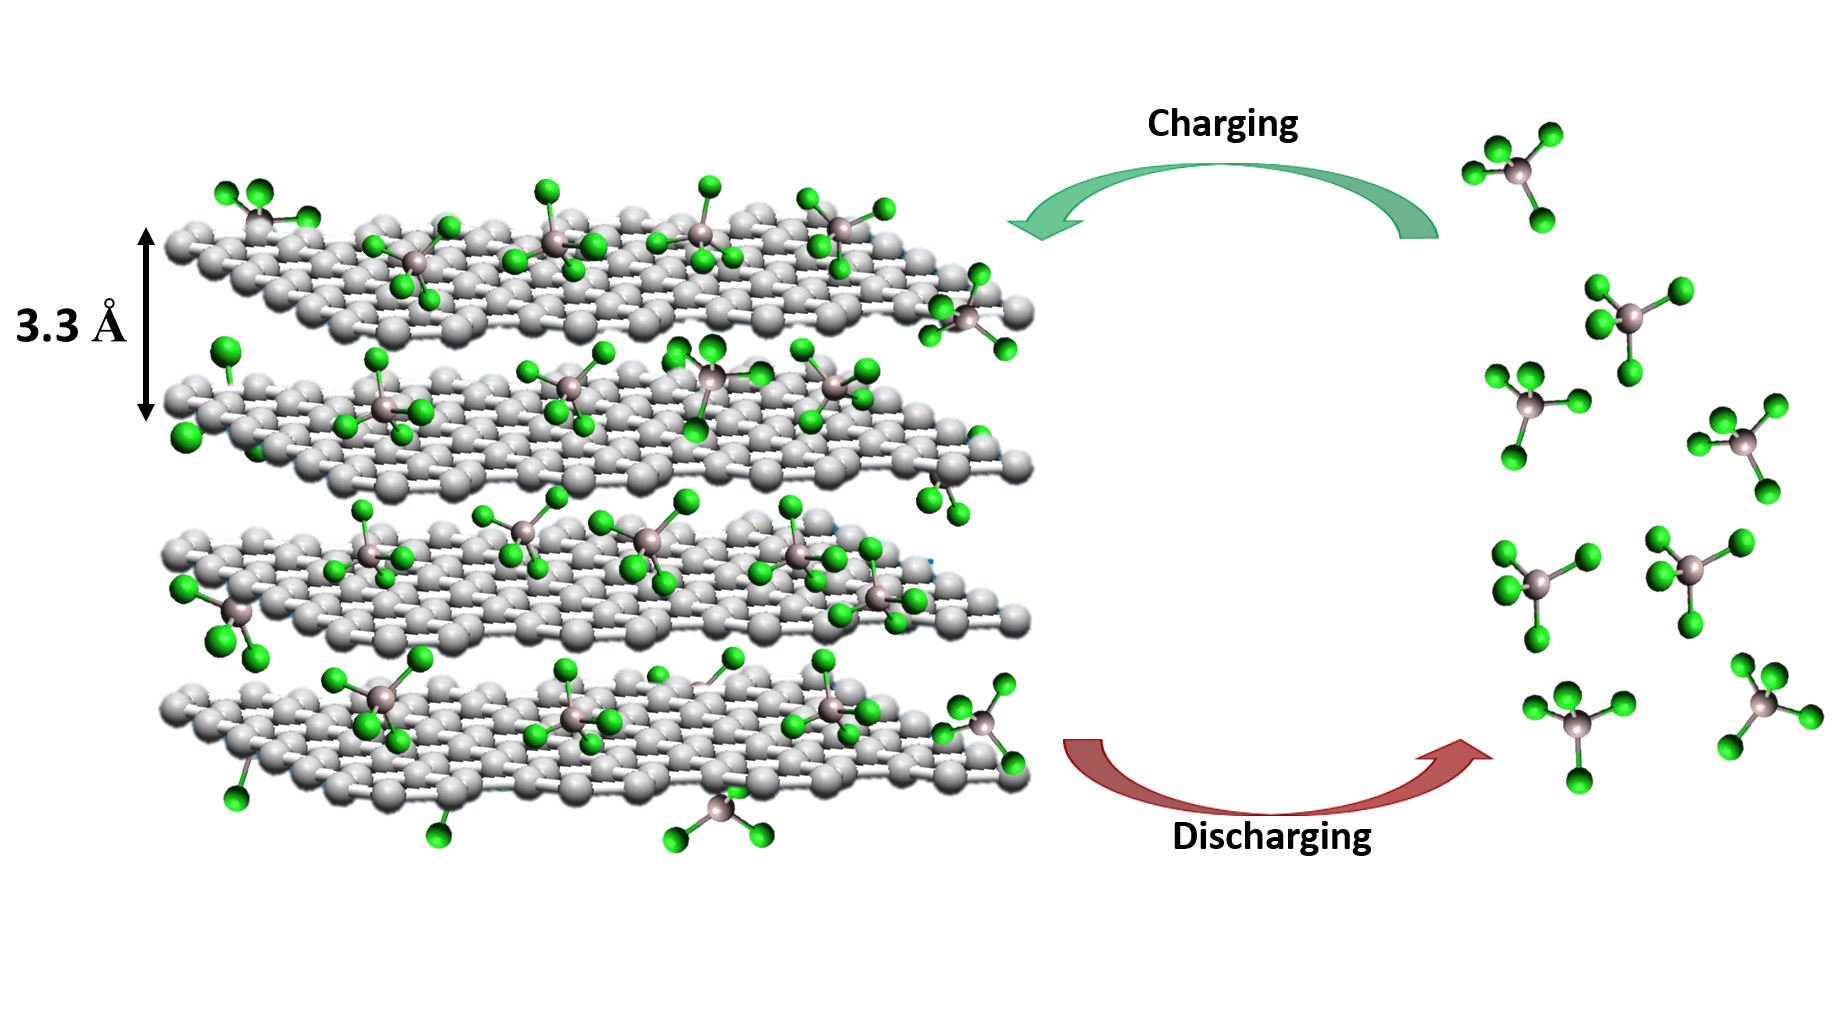
\includegraphics[width=\textwidth]{fig/graphitemech}
    \caption{Intercalation of \ce{AlCl4-} ions during charging and deintercalation during discharging in an Al/graphite cell. The interlayer distance between two graphite sheets is 3.3 \AA.}
  \label{fig:graphitemech}
\end{figure}

In this work, four different carbon-based materials --- Ac from human hair, AC from hemp fibers, fullerene extract (CFEx) and Super-P carbon black (Super-P) were investigated as cathodes for AIBs. Super-P is an amorphous form of carbon. It is highly conductive and is added in electrode slurries to enhance the conductivity of a cathode material. Activated carbon derived from natural products such as rice husk, coconut shells or wood, have been previously used in batteries and super-capacitors \cite{hussain_development_2019, frackowiak_carbon_2001}. Most of the carbon-based materials have a high surface area. AC derived from both hair and hemp fibers contain pores of various sizes (mesopores and micropores). Fullerenes on the other hand, has a tightly packed structure with Brunauer-Emmet and Teller (BET) surface area of 19 m$^2$ g$^{-1}$ \cite{}.

\section{Results and discussion}
The battery system comprised a cathode, 99\% pure Al foil as the anode, and a room temperature ionic liquid (RTIL) as the electrolyte. Super-P is an amorphous form of carbon with a high surface area of 62 m$^2$ g$^{-1}$ and a highly disordered structure \cite{see_reversible_2017}. The pore sizes range from $\sim$30-50 nm \cite{younesi_analysis_2015}. AC derived from human hair, hemp fibers, and SPCB all have a non-crystalline structure. However their Raman spectra revealed the presence of a few graphitic planes. These planes would allow \ce{AlCl4-} ions to intercalate during charging. CFEx (a mixture of \ce{C60} and \ce{C70} fullerenes) does not have a layered structure. Fullerenes have a cage-like morphology and the chloroaluminates are not small enough to move in and out of them during charge/discharge. We assumed that \ce{AlCl4-} anions migrated through the gaps present in between the fullerenes and interacted with their surface. Specific capacities and Coulombic efficiencies (CEs) of the cathodes were recorded at various current rates (cf.\ Figure \ref{fig:CDCall}a and b). Morphology of the cathodes before and after the cycles were studied using Raman spectroscopy, XRD patterns and scanning electron microscopy (SEM).

\begin{figure}[]
  \centering
  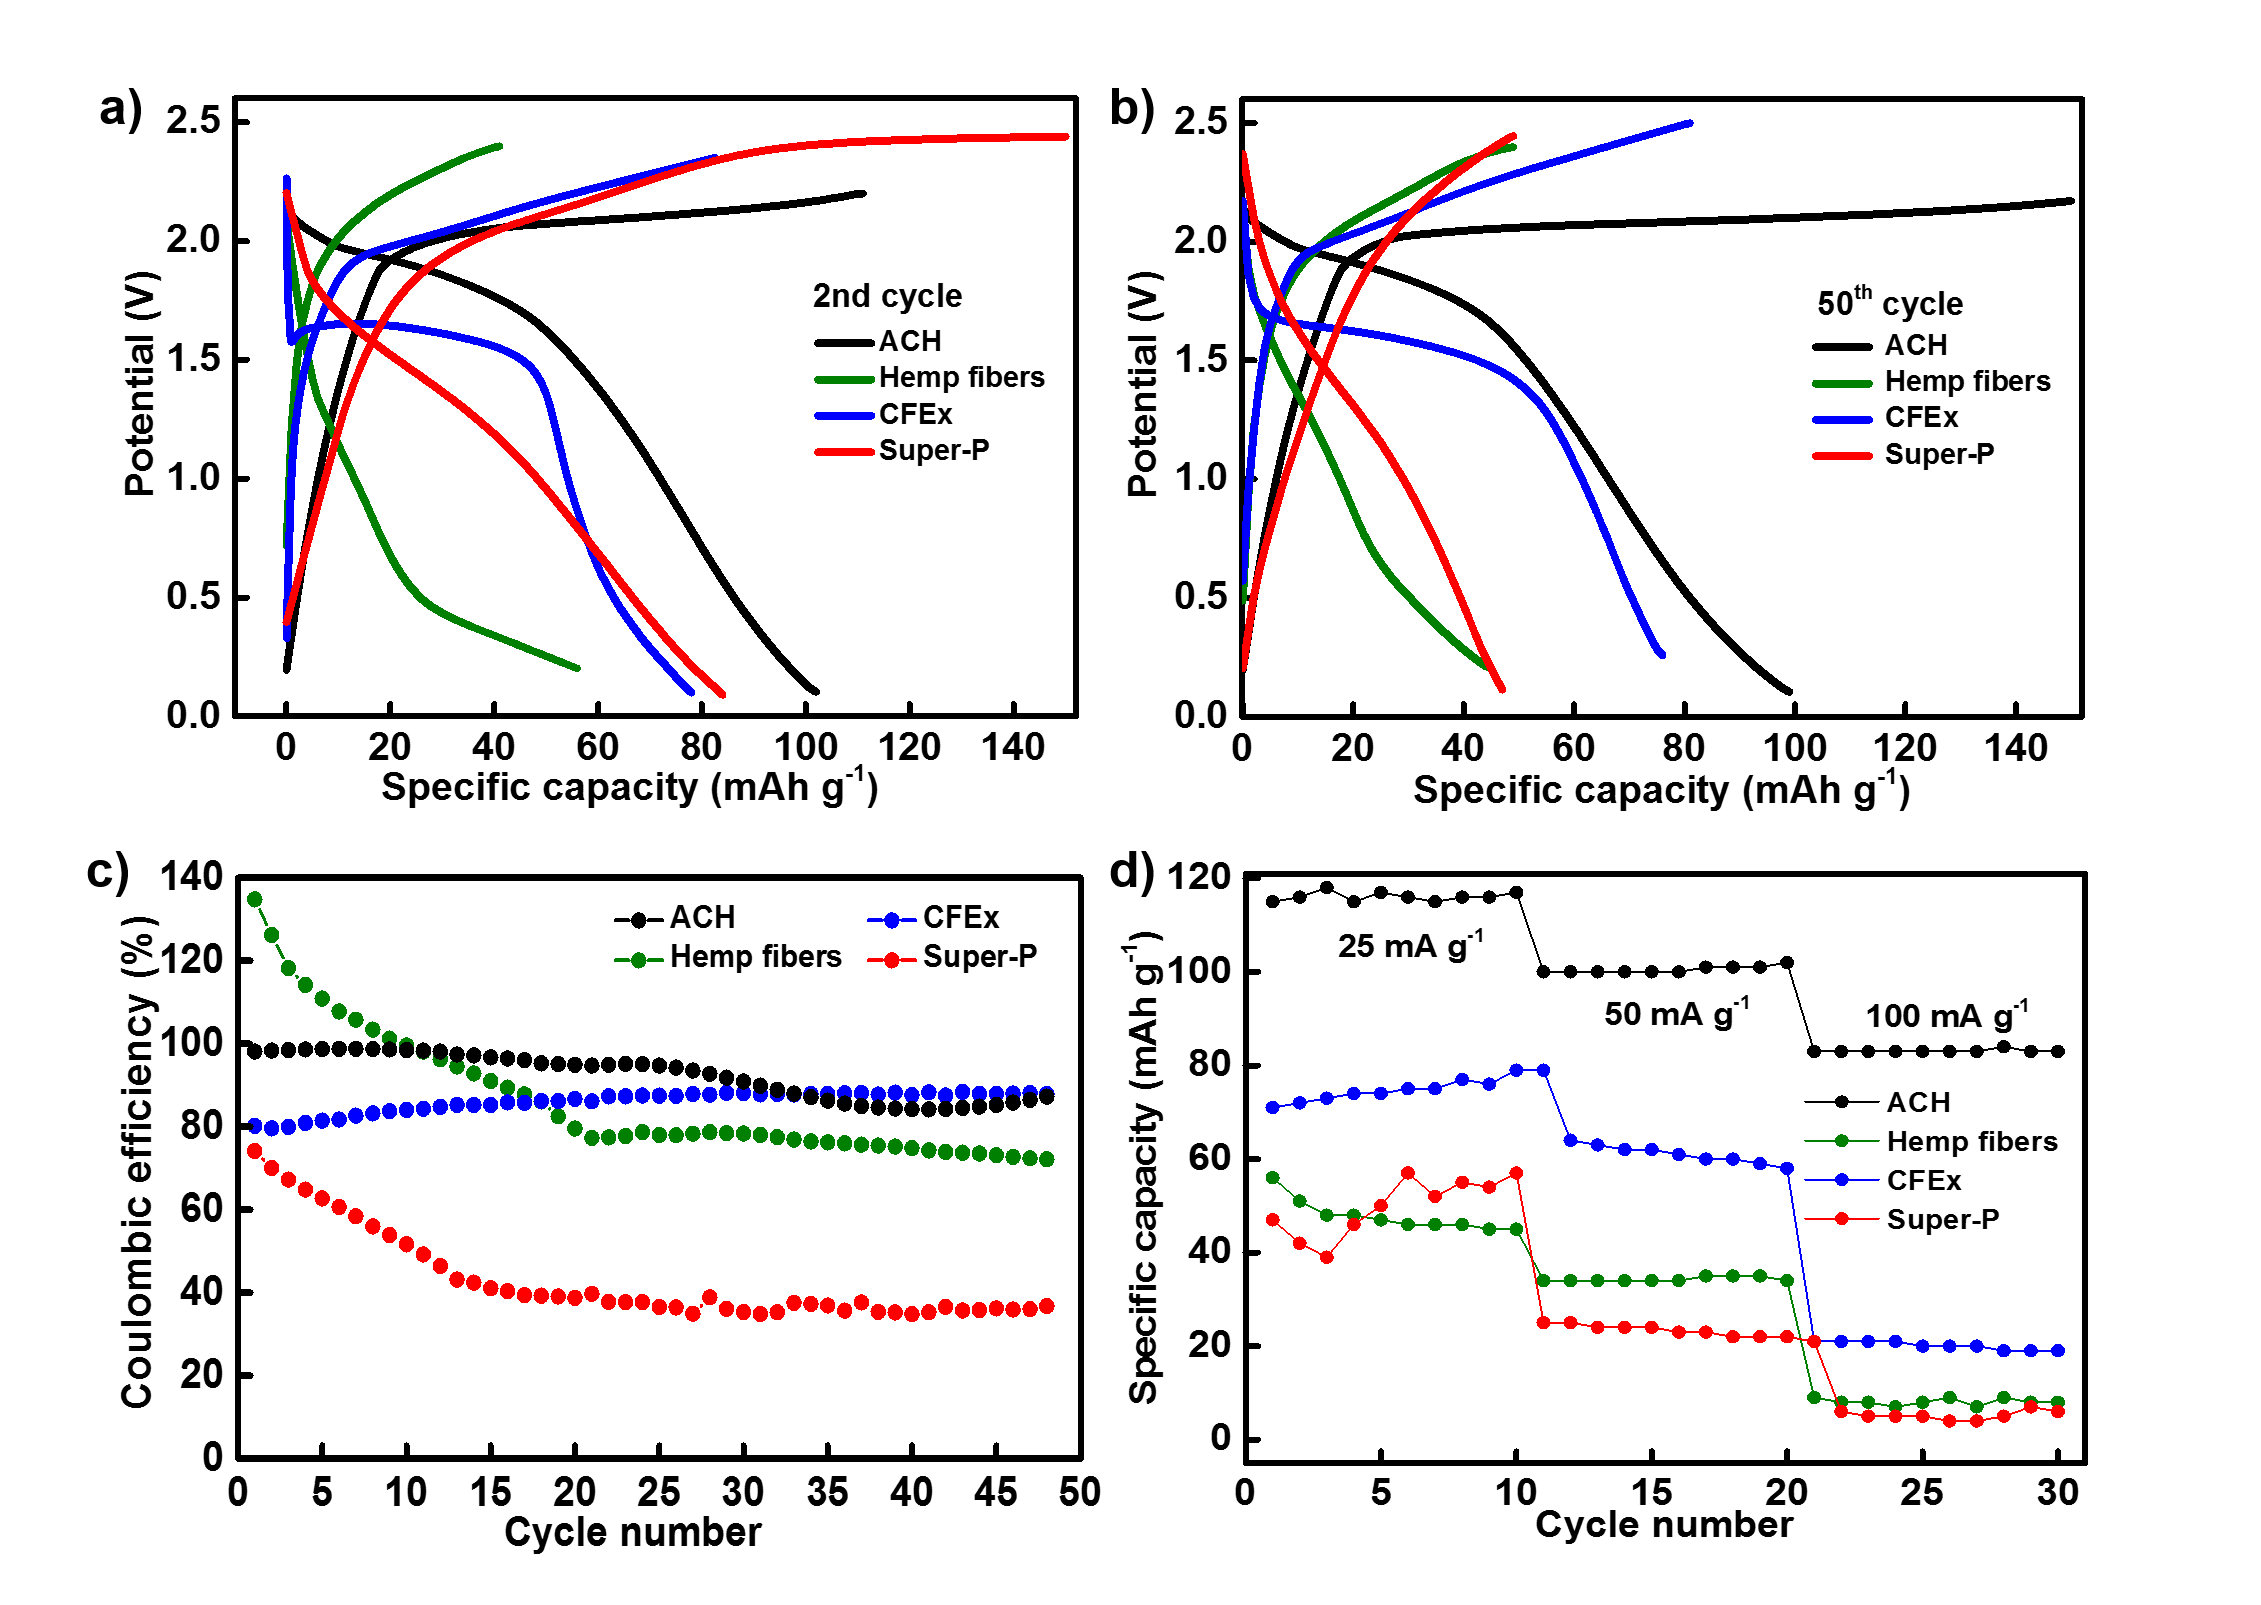
\includegraphics[width=\textwidth]{fig/CDCall}
    \caption{Specific capacities of AC (human hair, hemp fibers), CFEx and SPCB in their a) first and b) 50$^{th}$ cycle at a current rate of 50 mA g$^{-1}$. c) Coulombic efficiencies (CEs) of cells at a current rate of 50 mAg$^{-1}$. d) Galvanostatic charge/discharge profile of all cells at various current rates ranging from 25 mAg$^{-1}$ to 100 mAg$^{-1}$ in a two-electrode setup against Al$^{3+}$/Al.}
  \label{fig:CDCall}
\end{figure}

Figures \ref{fig:CDCall}a) and b) show the specific capacities of all cells for their first and 50$^{th}$ cycles. Human hair cathodes exhibited a high capacity of $\sim$100 mAh g$^{-1}$ with CE of $\sim$95\% shown in Figure \ref{fig:CDCall}c). Hemp batteries displayed a capacity of 56 mAh g$^{-1}$ in their first cycle, which decreased to 45 mAh g$^{-1}$ after 50 cycles. CFEx displayed a capacity of around 80 mAh g$^{-1}$ with CE of $\sim$90\% and maintained that for 50 cycles. With an initial value of 84 mAh g$^{-1}$, specific capacity of Super-P decreased to 47 mAh g$^{-1}$ and a low CE of $\sim$40\% was observed. The discharging capacity of SPCB and hemp fibers decreased considerably after repeated charge/discharge cycles. A low CE that was observed in both hemp and Super-P, can be attributed to side reactions in the batteries. These may include electrode or electrolyte interactions with impurities or degradation of the cathode structure (pulverisation) \cite{gyenes_understanding_2015-1}. The capacity loss for CFEx and human hair cells was minimal. This suggests that CFEx and human hair have a more stable structure and have the potential to store charge reversibly \cite{pramanick_human_2016}.

\section*{Activation of carbon}
The production of AC consists of carbonisation of a precursor at a temperature below 900$^{\circ}$ C in an inert atmosphere and chemical or physical activation of the carbonised precursor. Activating agents play an important role in determining the porosity of AC \cite{arenas_effect_2004}. Using alkali hydroxides at high temperature creates micropores, which increases the surface area of the material \cite{dong_commercial_2019, liu_hair-based_2017}. In this work, sodium hydroxide (NaOH) was used as the activating agent. The following reaction is taking place within the carbon matrix after addition of NaOH:

\begin{center}
    4NaOH + C $\longrightarrow$ 4Na + 4\ce{CO2} + 2\ce{H2O} \cite{satish_macroporous_2015}
\end{center}

\begin{figure}%[ht!]
\centering
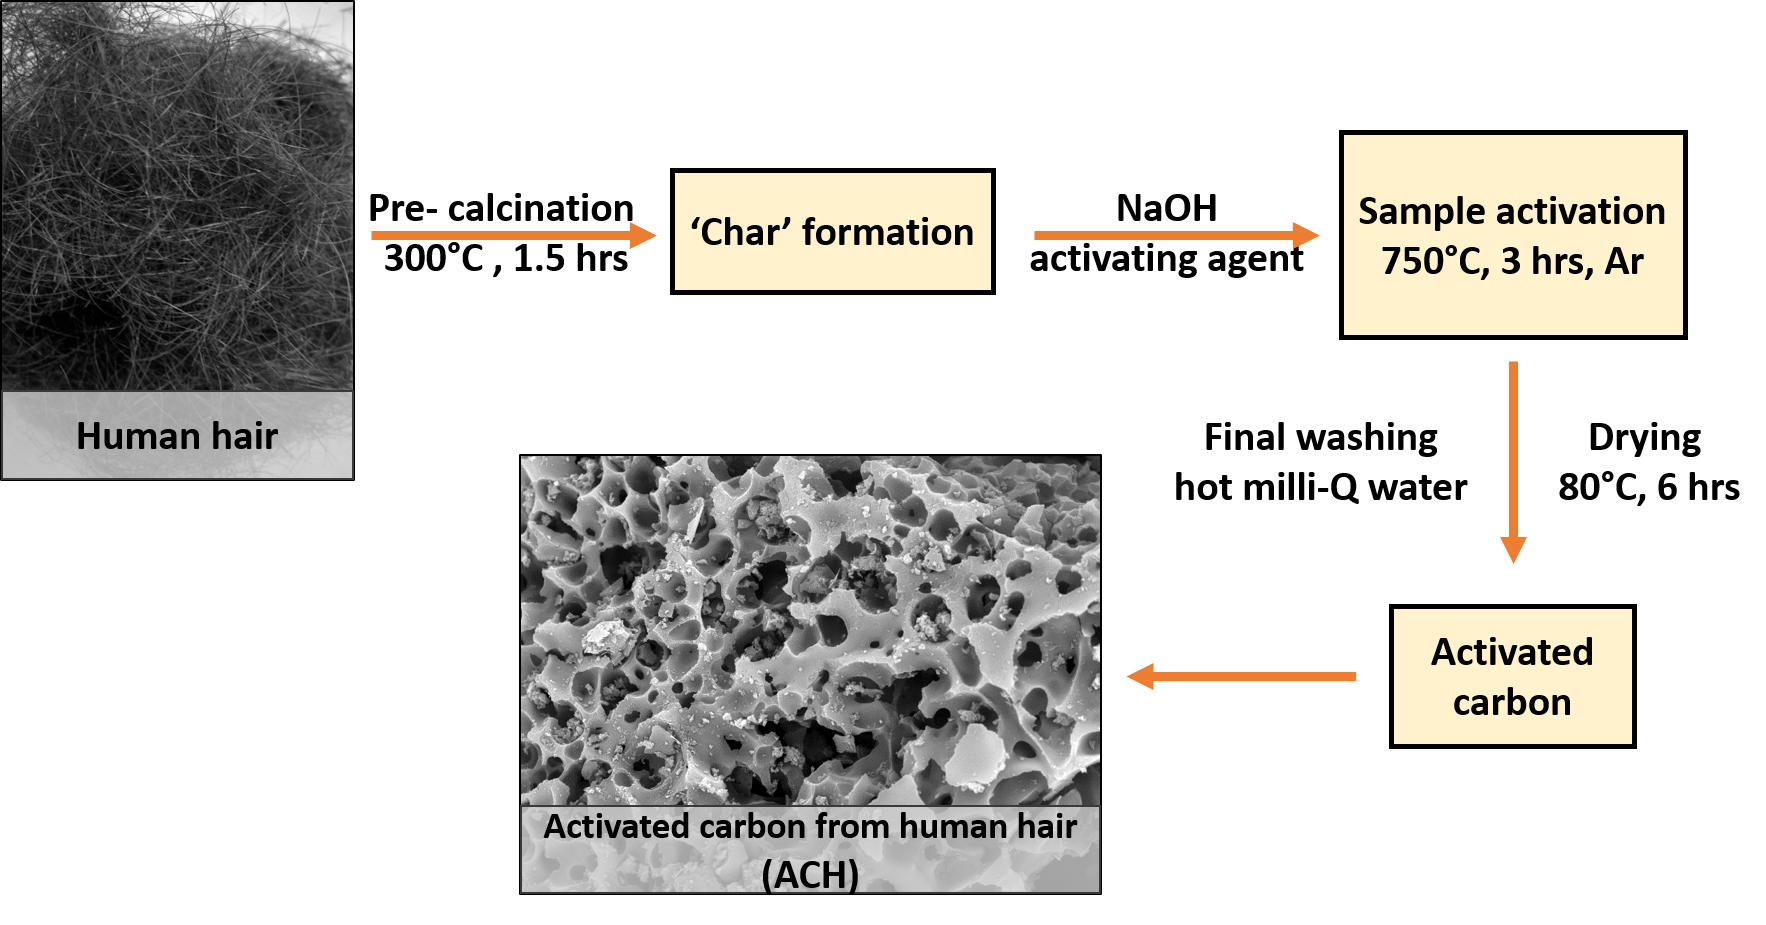
\includegraphics[width=\textwidth]{fig/ACHsyn}
\caption{Synthesis of activated carbon (AC) from human hair using NaOH as the activating agent.}
\label{fig:ACHsyn}
\end{figure}

% Paragraph above: you need to prove/reason every statement that you make. You just claim a lot of stuff without providing any evidence. Also: ARTICLES!!!!!
Fullerenes have a fused-ring structure with a nucleus-to-nucleus diameter of 7.1\AA\ and a van der Waals (vdW) diameter of 11\AA\ in a single crystal. However, they are zero-dimensional materials, which means they cannot provide an efficient path for electron transport or a long-range conductivity \cite{loutfy_fullerene_2002, winkler_two-component_2007}. They are known to be weak battery materials owing to their solubility in electrolytes, especially in LIBs \cite{seger_prospects_1991}. To test their solubility in \ce{AlCl3}-EMImCl, 100 mg of CFEx were mixed in the electrolyte and stirred for 24 hours. The solution was left to stand for another 24 hours inside a \ce{N2}-filled glove box. CFEx seemed to dissolve in the RTIL (Figure \ref{fig:CFExsol}) since no phase separation was observed. It has been reported that poly-sulphides (formed during charge/discharge cycles) are soluble in the electrolyte of a Li-S battery. They form an insulating layer of \ce{Li2S} on the anode, which results in capacity fading \cite{sun_effect_2017}. Since no such effect was observed in the fullerene cells, this phenomena does not seem to impact its charge-storing capacity. On the contrary, Al/CFEx cells demonstrated excellent capacity retention at various current rates (Figure \ref{fig:CDCall}d)).   

\begin{figure}
\centering
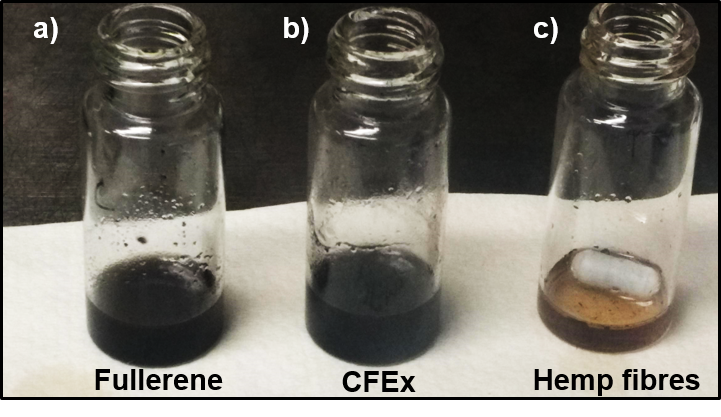
\includegraphics[width=0.75\textwidth]{fig/CFExsol}
\caption{Comparison of solubility of a) pure \ce{C60} fullerene b) fullerene extract (CFEx) and AC derived from hemp fibers in \ce{AlCl3}/EMImCl ionic liquid electrolyte.}
\label{fig:CFExsol}
\end{figure}

It has been previously established that chloroaluminates intercalate into the graphitic planes during charging \cite{lin_ultrafast_2015-2}. Since both AC and SPCB cathodes contain graphitic planes, we expected intercalation during cell charging. To study these changes, charged cathodes of all materials were analysed by Raman spectroscopy and compared with the pristine ones. The data obtained is displayed in Figure \ref{fig:raman}. Graphite shows a characteristic D-band present at 1300 cm$^{-1}$, which originates from the hybridized vibrational modes associated with graphene edges and indicates the absence of long-range order. Pristine hair, hemp and SPCB cathodes showed a significant D-band present at $\sim$1300 cm$^{-1}$ for human hair, 1329.7 cm$^{-1}$ for hemp fibers, and 1352.0 cm$^{-1}$ for SPCB, indicating the absence of a defined lattice structure. Both the peaks at 1600 cm$^{-1}$ and 1350 cm$^{-1}$ are broad due to the presence of \ce{sp2} clusters like $\alpha$-carbons, which have a bond angle disorder \cite{shimodaira_raman_2002}.

 \begin{figure}
  \centering
  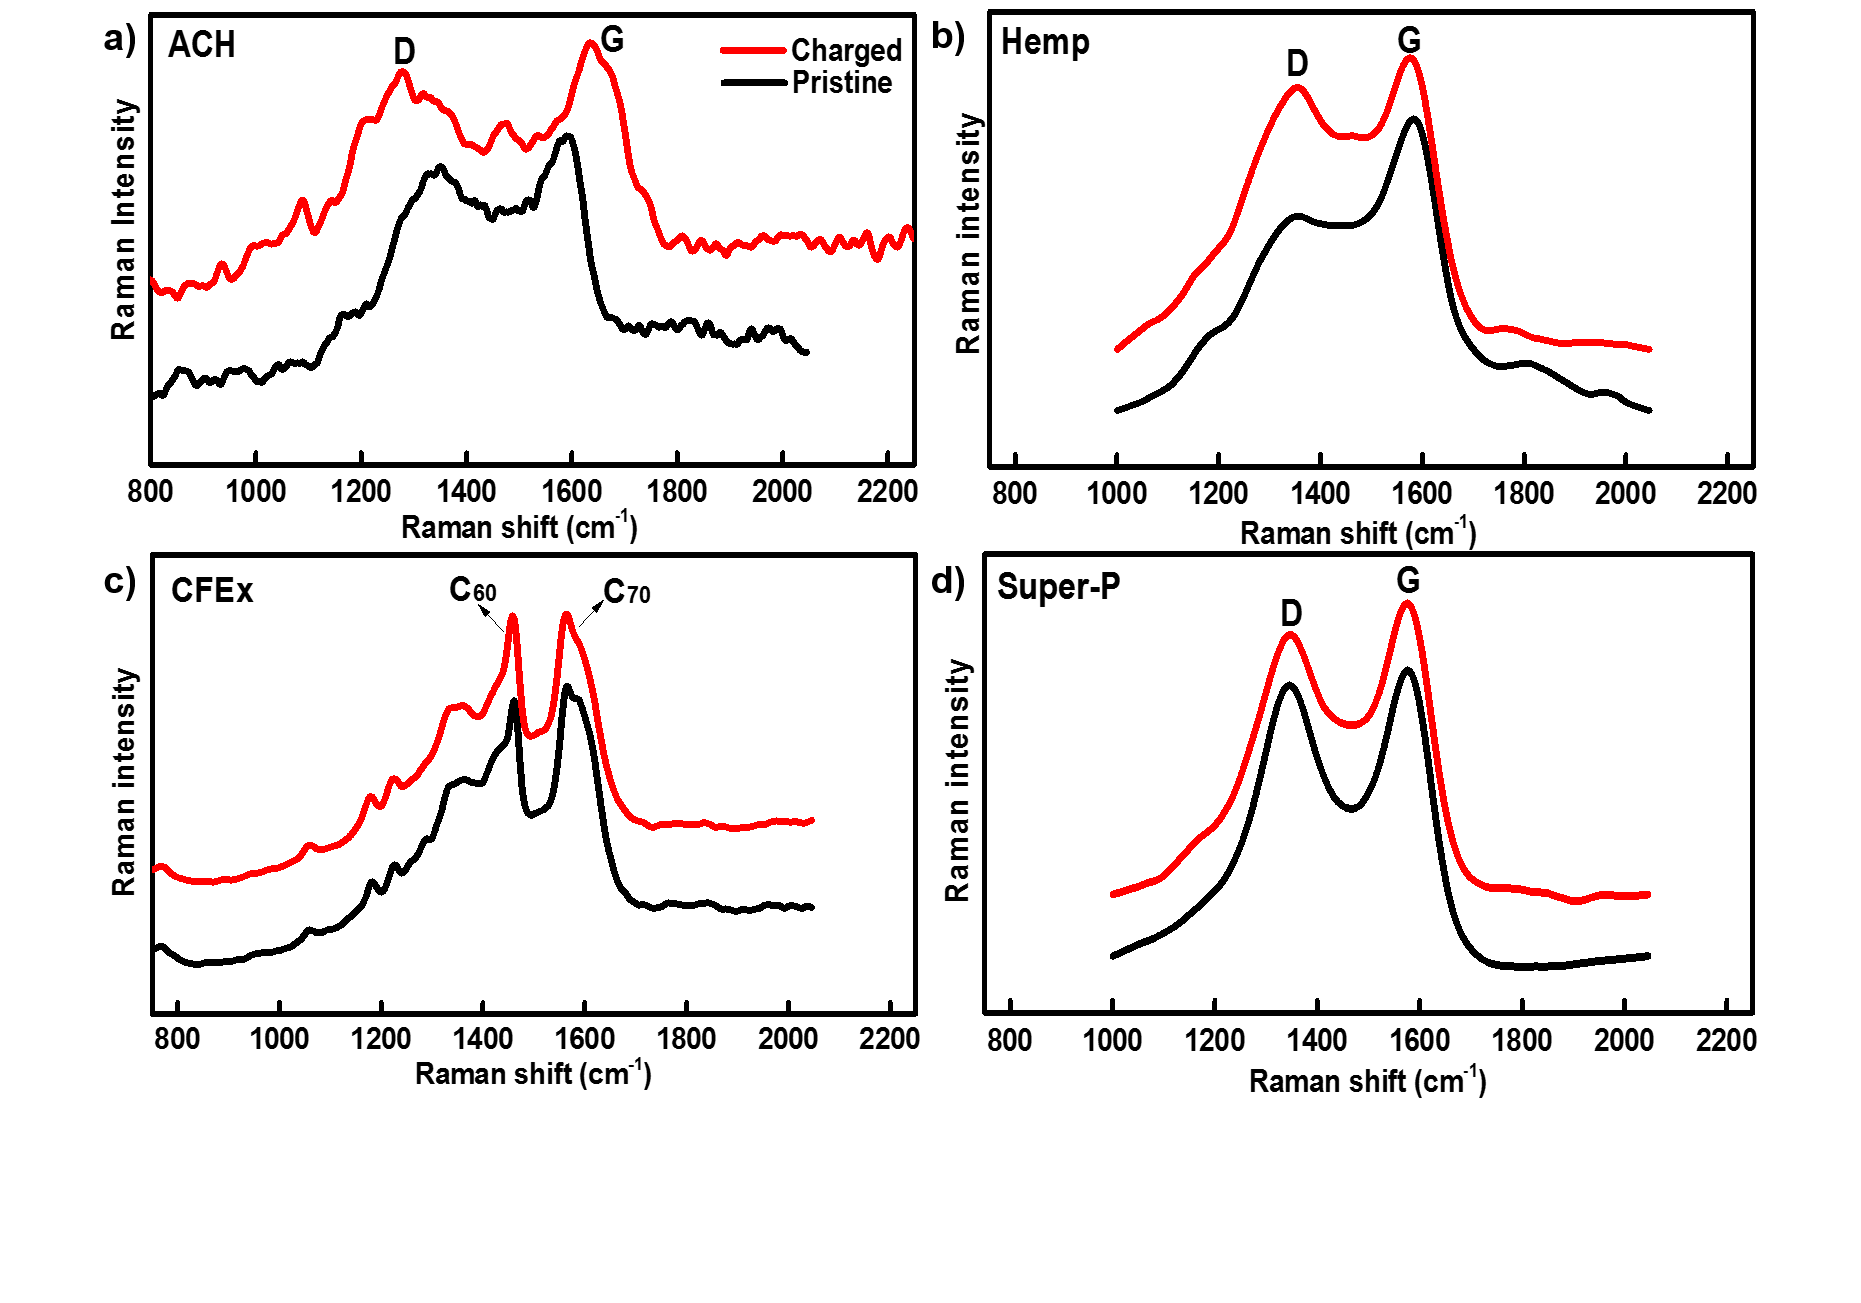
\includegraphics[width=\textwidth]{fig/raman}
    \caption{Raman spectra of pristine (in black) and charged (in red) a) CFEx, b) AC from hemp fibers, c) from human hair (ACH) and d) Super-P cathodes displaying presence of both D and G bands.}
  \label{fig:raman}
\end{figure}

Raman spectra of CFEx in Figure \ref{fig:raman}c) displayed the characteristic bands of both \ce{C60} and \ce{C70} molecules. A 'pentagonal pinch mode', usually observed in a \ce{C60} Raman spectrum, was present at 1460 cm$^{-1}$. It was observed that \ce{C70} had multiple bands. This was due to its reduced molecular symmetry, which increased the number of vibrational modes, consequently increasing the number of active Raman bands \cite{kimbrell_analysis_2014}. It was interesting to note that the spectra of charged CFEx looked almost identical to the pristine ones. The results suggested that the fullerenes did not undergo any significant structural change during the cycles. As a result, the cells displayed a very stable CE. Furthermore, fullerenes stored the same amount of charge after every cycle (similar discharge capacity after 50 cycles) without undergoing any significant structural changes.

Charged AC (from hair) cathodes showed an increased full-width at half maxima (FWHM), which suggested an increase in the lattice defects and structure deformities. These defects would arise if the chloroaluminate ions intercalated into the few graphitic planes present in the carbon matrix. However, a highly porous structure would also allow surface adsorption of charge carrying species much like in super-capacitors \cite{beguin_carbons_2014}. Since activated carbon lacks the long-range ordered structure present in natural graphite, intercalation into short-range graphitic planes, as well as surface adsorption of chloroaluminates, can contribute to its high capacity \cite{brezesinski_ordered_2010}. This might have resulted in aluminium-hair batteries performing better than other materials by storing more charge as a result of the dual mechanism. A schematic of the proposed mechanism of an aluminium-hair battery is displayed in Figure \ref{fig:ACHmech}.

 \begin{figure}%[h!]
  \centering
  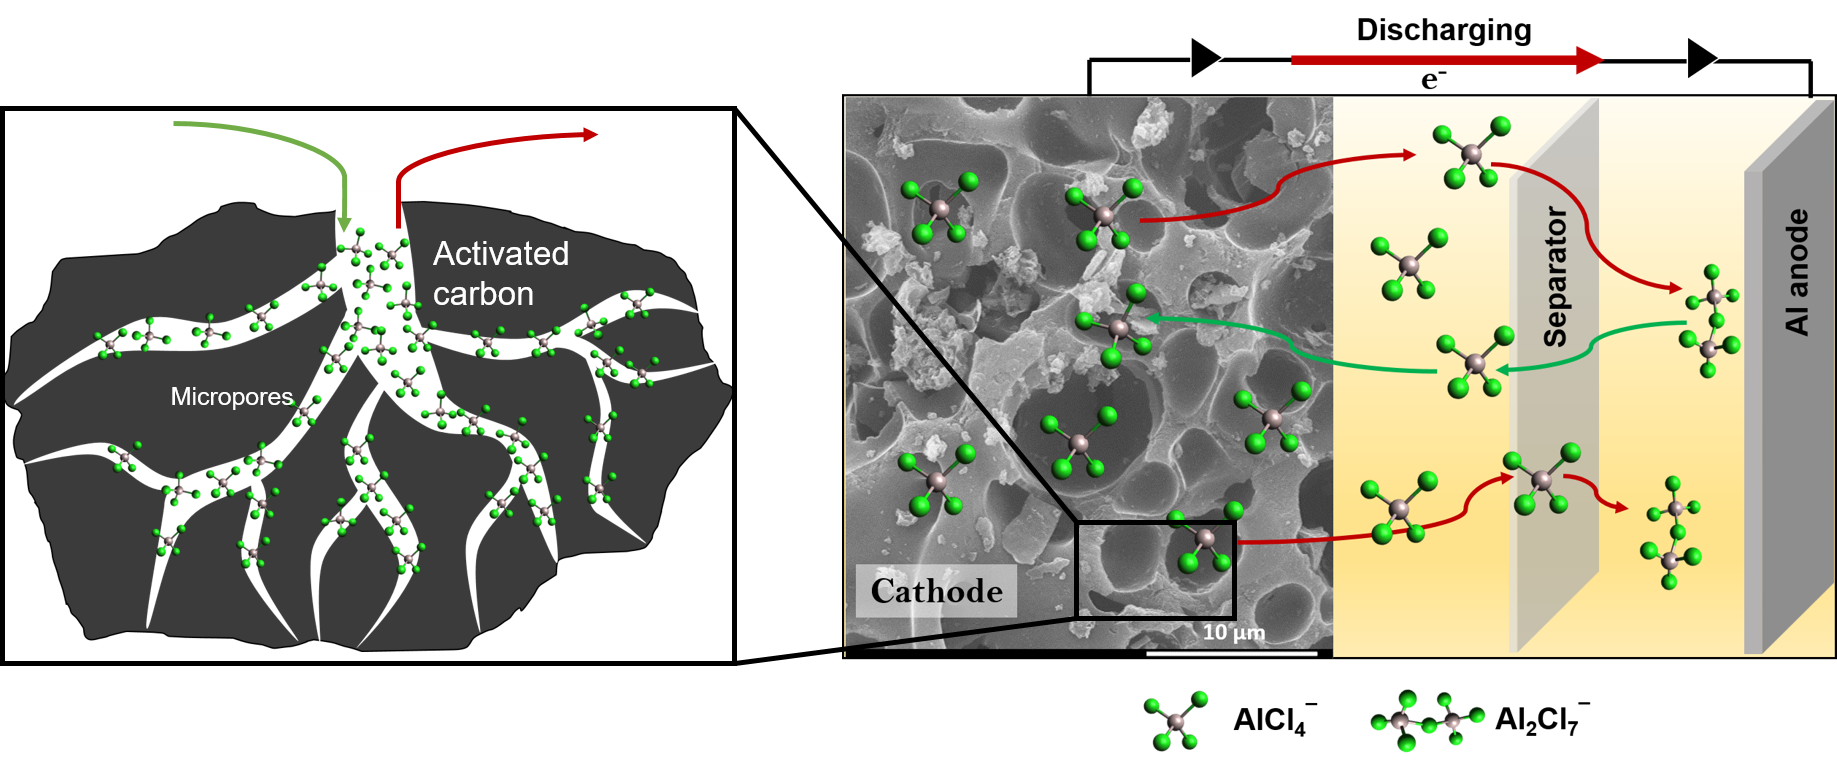
\includegraphics[width=\textwidth]{fig/ACHmech}
    \caption{Suggested mechanism for an Al/hair cell. Chloroaluminate ions (\ce{AlCl4-}) intercalate into the few graphitic planes and micro/mesopores present in them, in addition to surface adsorption of ions displaying both Faradaic and non-Faradaic processes for charge storage.}
  \label{fig:ACHmech}
\end{figure}

%contains about 51\% carbon, 17\% nitrogen, 21\% oxygen, 6\% hydrogen, 5\% sulfur, and trace amounts of iron, magnesium, arsenic, chromium and various minerals \cite{lee_chemistry}.

Figure \ref{fig:allmech}b) and c) show the proposed mechanism of charge storage in an Al/hemp and Al/SPCB cell. Both hemp fibers and SPCB had a highly disordered structure to begin with (cf.\ Raman spectra). Repeated intercalation or adsorption of ions onto their surface during the first few cycles further damaged their structure, which is one of the reasons why hemp and SPCB batteries failed to retain their capacity. However, CFEx does not have graphitic planes to intercalate chloroaluminate ions. Since the fullerenes have a very high surface area, surface adsorption of ions is highly likely \cite{adams_van_1994}. Furthermore, it might be possible for the anions to seep through the gaps present in between two fullerenes (\ce{C60} and \ce{C70}) as shown in Figure \ref{fig:allmech}a) and for the surface-based redox processes to take place in a systematic way throughout the electrode.

\begin{figure}
  \centering
  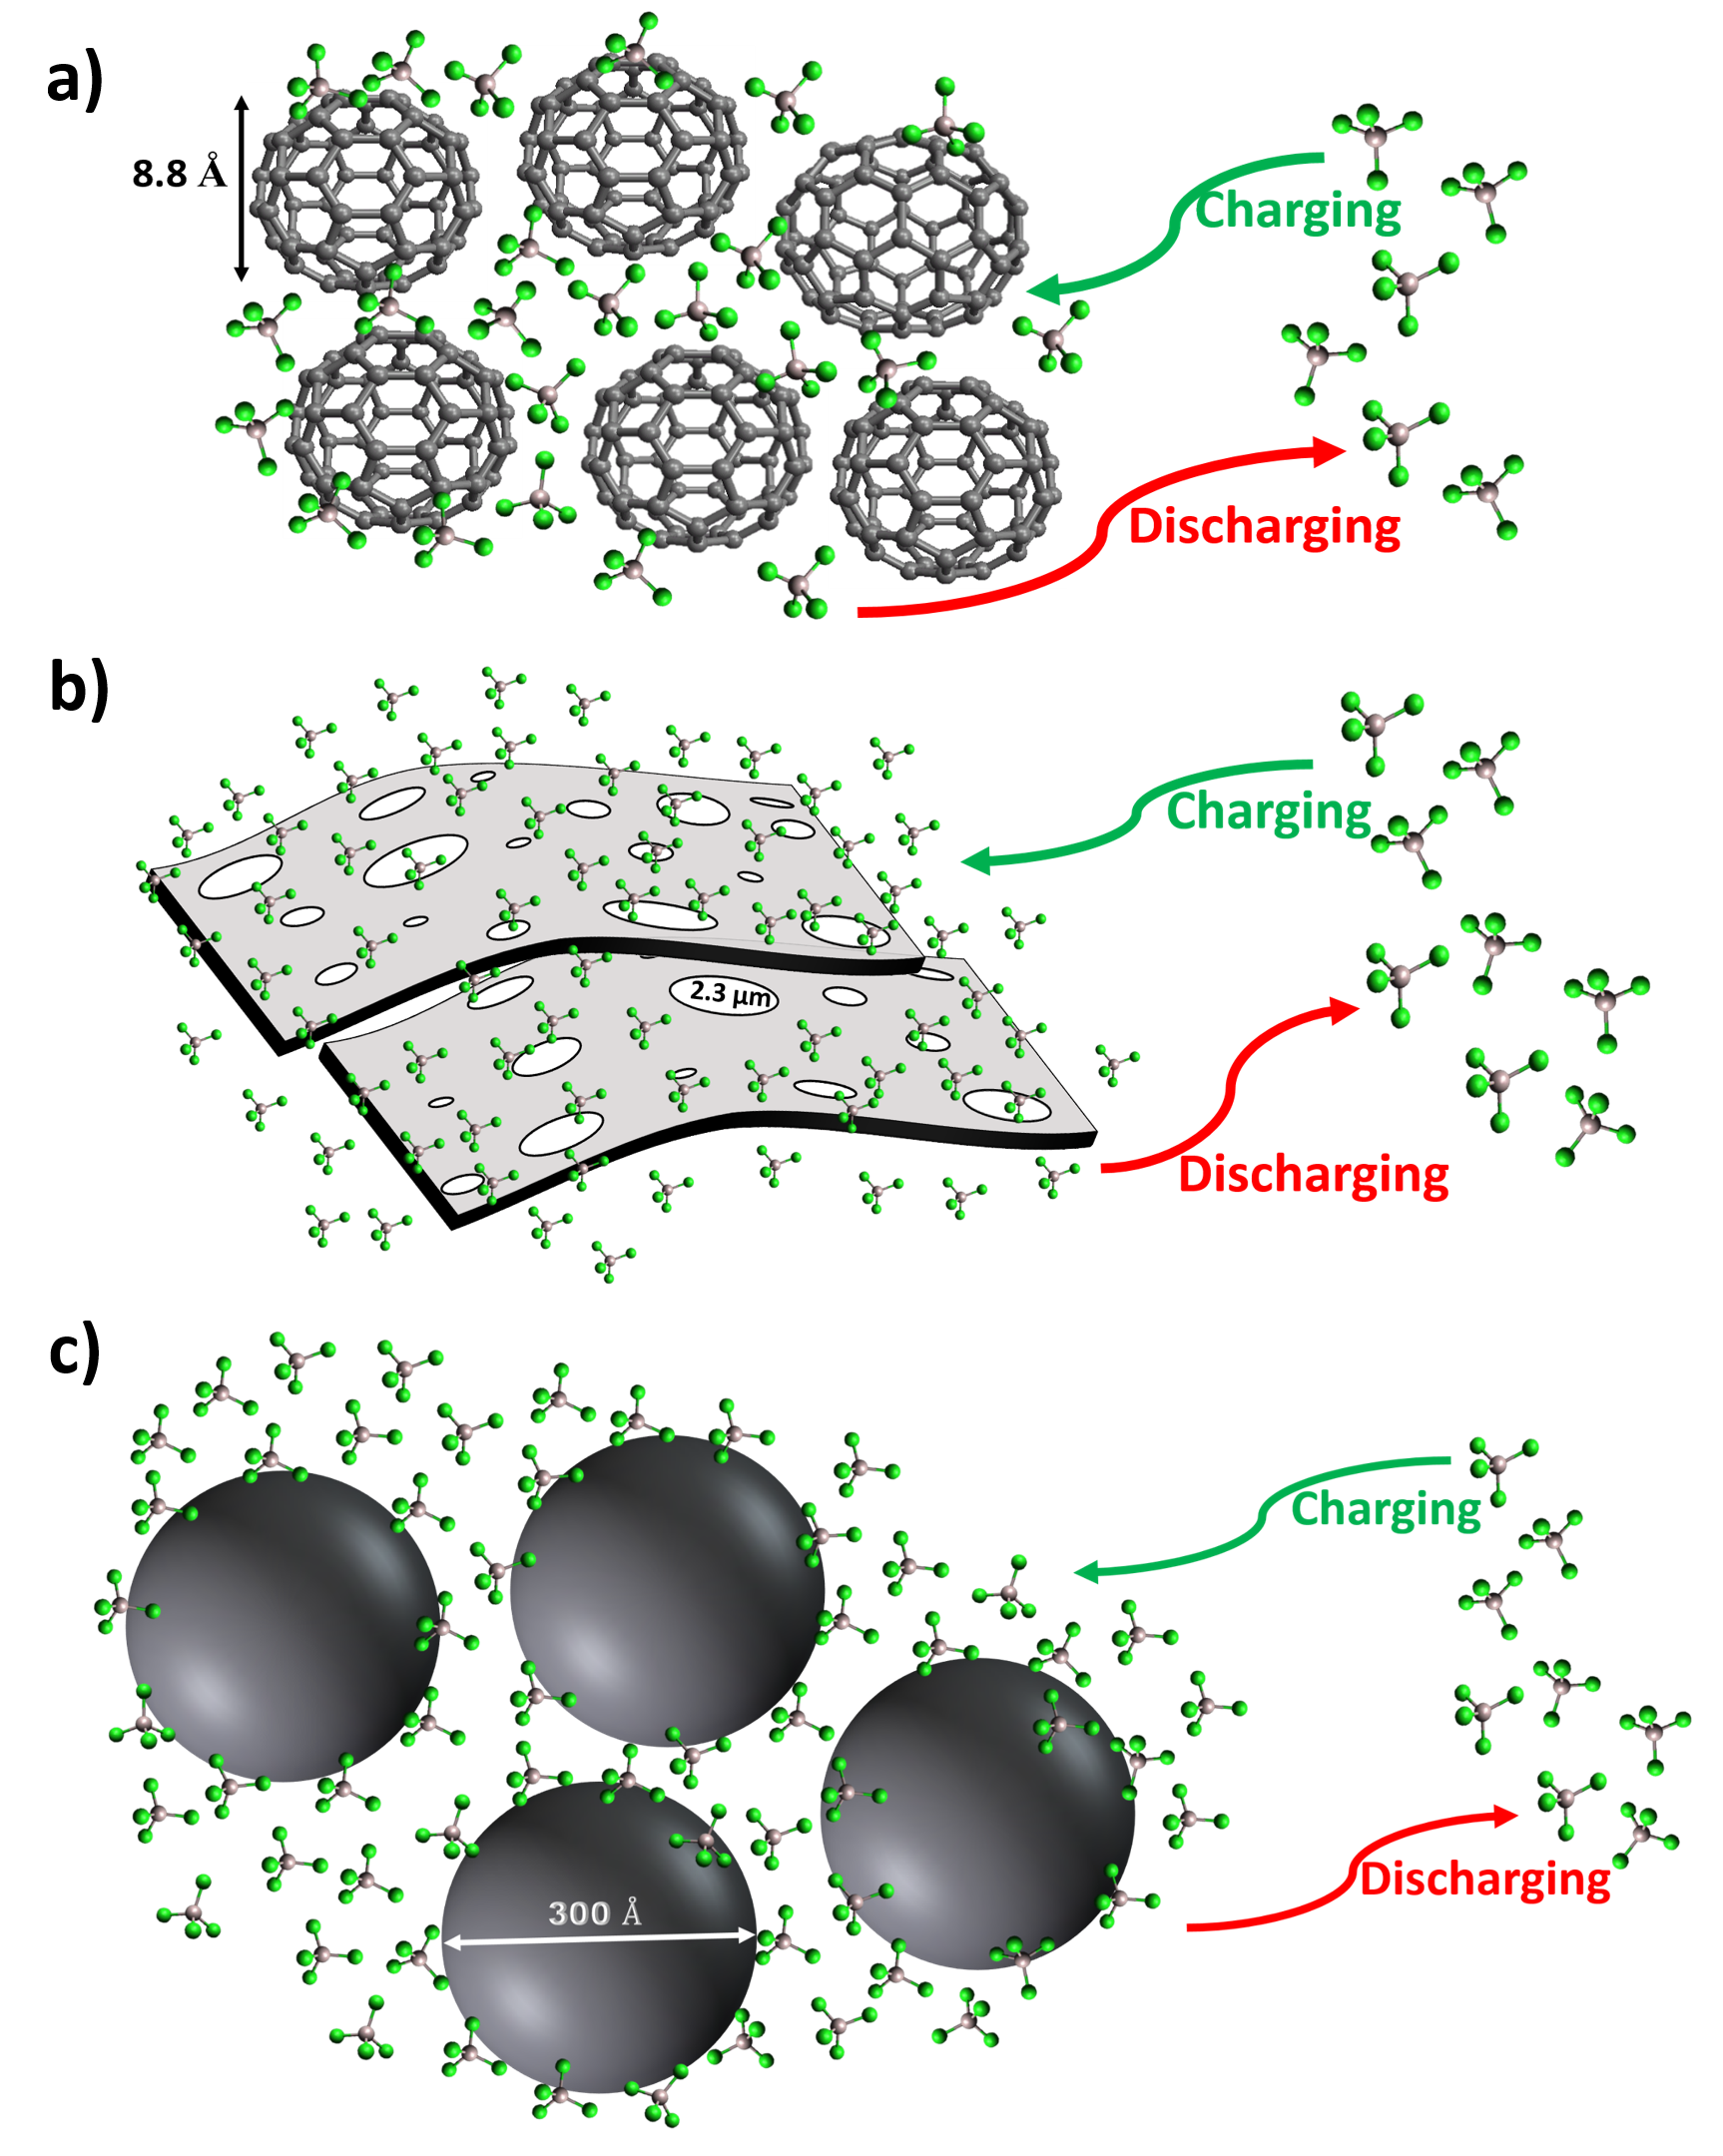
\includegraphics[width=\textwidth]{fig/allmech}
    \caption{Suggested mechanism for an a) Al-CFEx cell, b) Al-hemp cell, hemp fibers have pore sizes as large as 2.0-2.5 $\mu$m allowing the \ce{AlCl4-} to get absorbed on their surface. However, agglomeration of these fibers after a few cycles reduces the number of active sites available for effective charge storage, and c) Al-Super-P cell, chloroaluminates intercalate into the very few graphitic planes in Super-P, while few anions adsorb onto its surface. However, further cycling leads to cathode pulverisation, which results in capacity fading.}
  \label{fig:allmech}
\end{figure}

Figure \ref{fig:SEM} shows the SEM images of pristine (Figure \ref{fig:SEM}a), b), c) and d)) and charged (\ref{fig:SEM}e) ,f) ,g) and h)) cathodes of all carbon materials. Human hair and hemp fibers have a highly porous structure as seen in Figure \ref{fig:SEM}b) and d). However, hemp lost its surface porosity after 30 cycles, Figure \ref{fig:SEM}f). In addition, Figure \ref{fig:SEM}d) and h) implies that SPCB underwent significant agglomeration during cycles. It was interesting to note that the fullerene cathode retained its morphology after 50 cycles. 

\begin{figure}
  \centering
  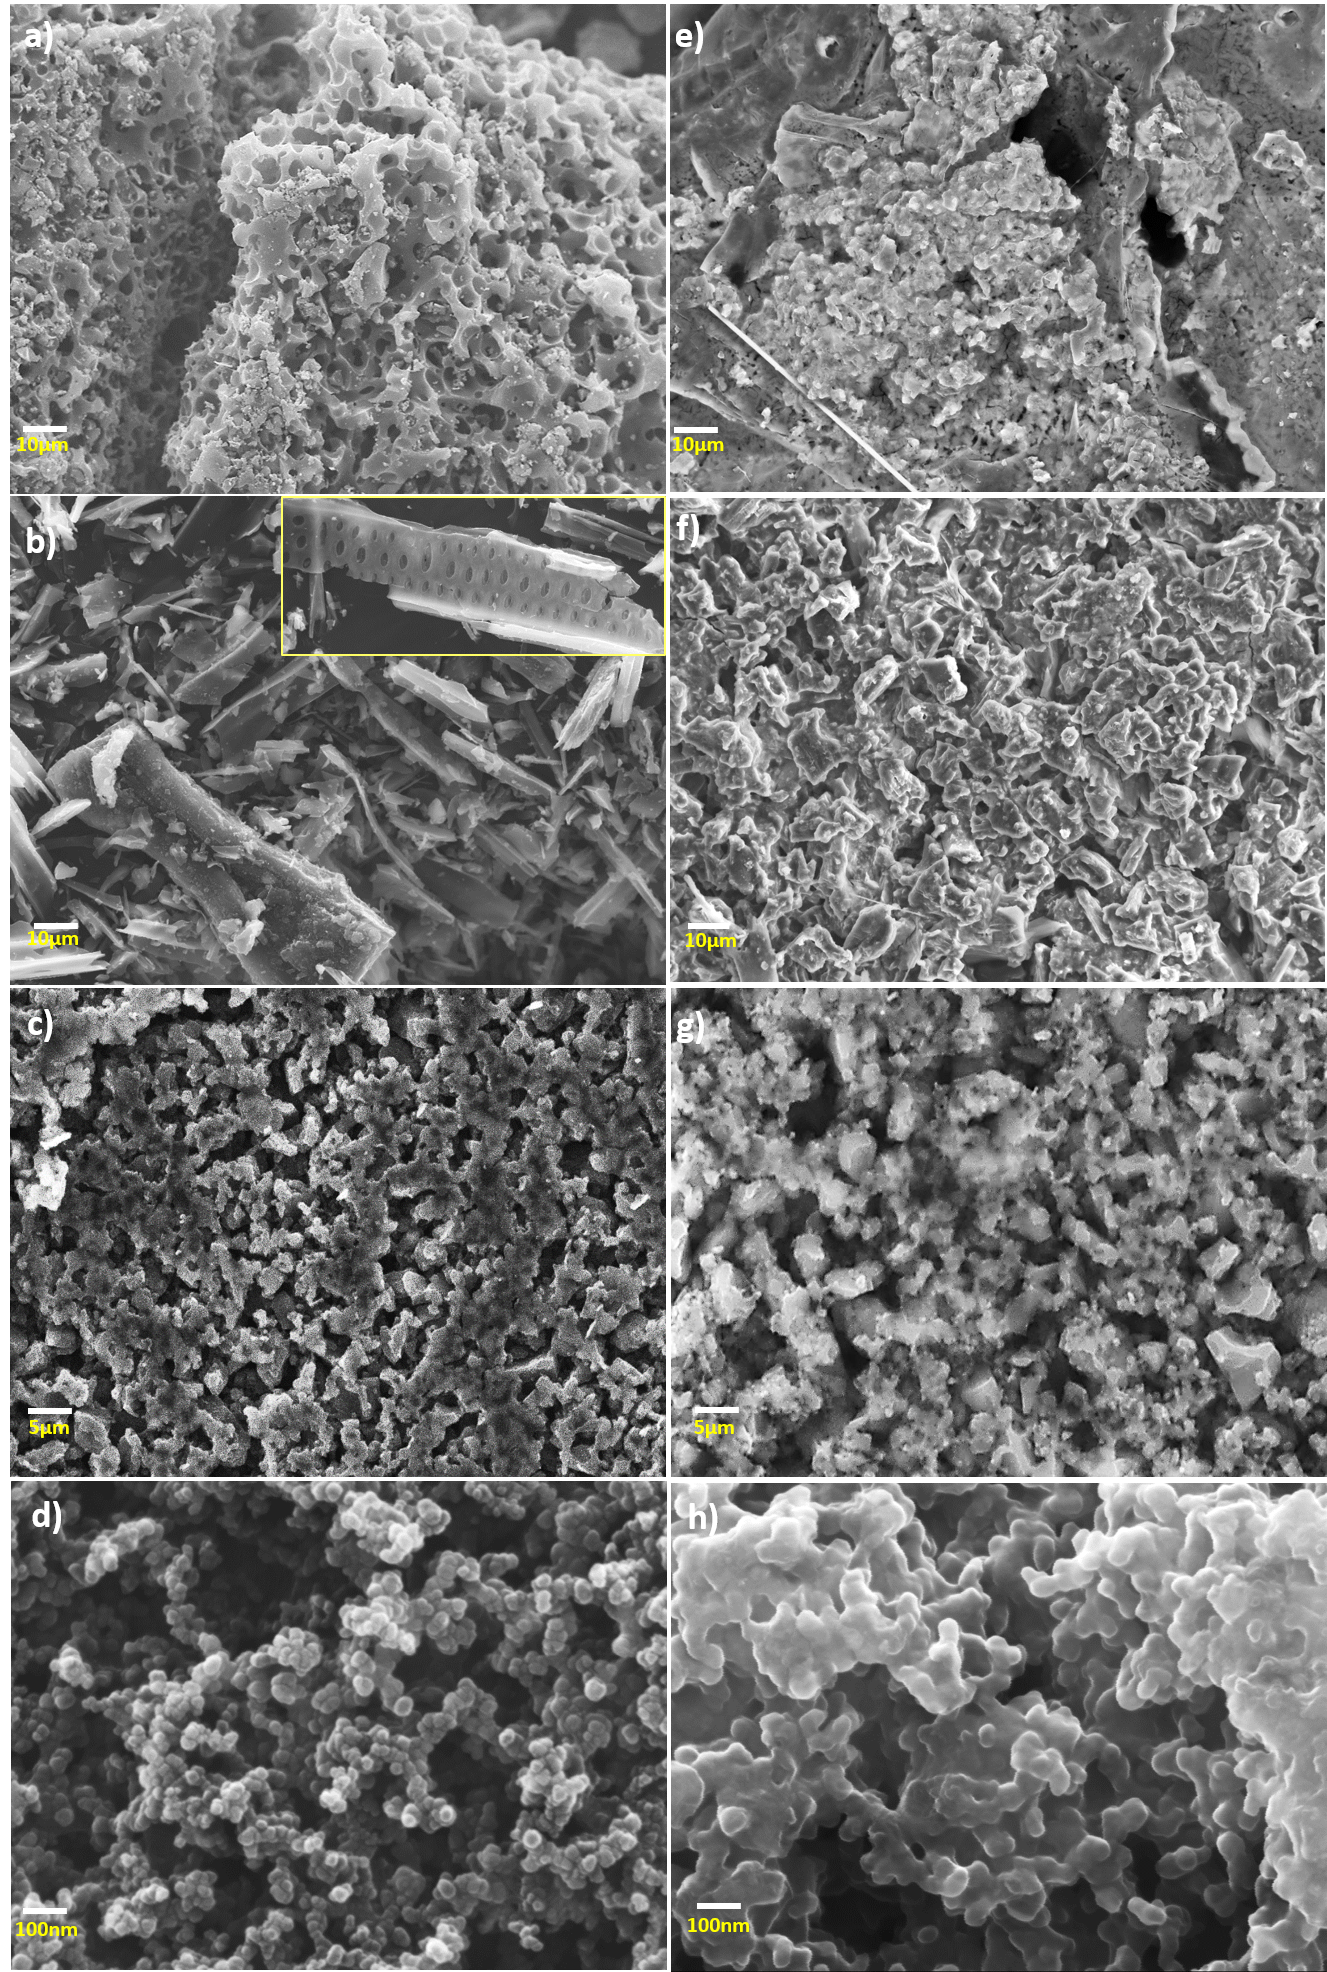
\includegraphics[width=0.8\textwidth]{fig/SEM}
    \caption{Scanning electron microscopy (SEM) images comparing pristine a) human hair, b) hemp, c) CFEx and d) SPCB and charged e) human hair, f) hemp, g) CFEx and h) SPCB cathodes. Hemp fibers and SPCB undergo permanent changes after charge/discharge cycles and fail to retain capacity.}
  \label{fig:SEM}
\end{figure}

Pristine (in black), charged (in green) and discharged (in red) cathodes of CFEx and human hair are showed in Figure \ref{fig:XRD}a) and b) respectively. Figure \ref{fig:XRD}a) displays the characteristic peaks of both \ce{C60} and \ce{C70} at 2$\theta$ values of 10.9$^{\circ}$, 17.8$^{\circ}$, 20.9$^{\circ}$ and 28.2$^{\circ}$ for \ce{C60} and 18.9$^{\circ}$, 19.3$^{\circ}$ and 21.8$^{\circ}$ for \ce{C70} molecules. New diffraction peaks at lower 2$\theta$ values appeared for charged electrodes. However, after discharge, the XRD patterns looked similar to the ones of the pristine cathodes. This data strongly suggests a reversible process taking place during cycling. To confirm this, the unit cell lattice parameters for both pristine and charged cathodes using \ce{C60} were calculated. The unit cell had a tetragonal crystal symmetry with a space group of \textit{P42/ mmc} and a space group number 131 (ICDD: 04-013-1339). Lattice parameters 'a' and 'b' for the charged cathode increased from 9.06 \AA\ to 9.57 \AA\ and 'c' increased from 15.03 \AA\ to 15.65 \AA, as shown in Figure \ref{fig:cfexcrys}a) and b). Lattice parameters of a discharged fullerene were closer to pristine values. These changes suggested a reversible insertion of chloroaluminates into the free spaces between fullerene molecules taking place. A possible site for \ce{AlCl4-} intercalation is depicted in Figure \ref{fig:cfexcrys}c). 

\begin{figure}
  \centering
  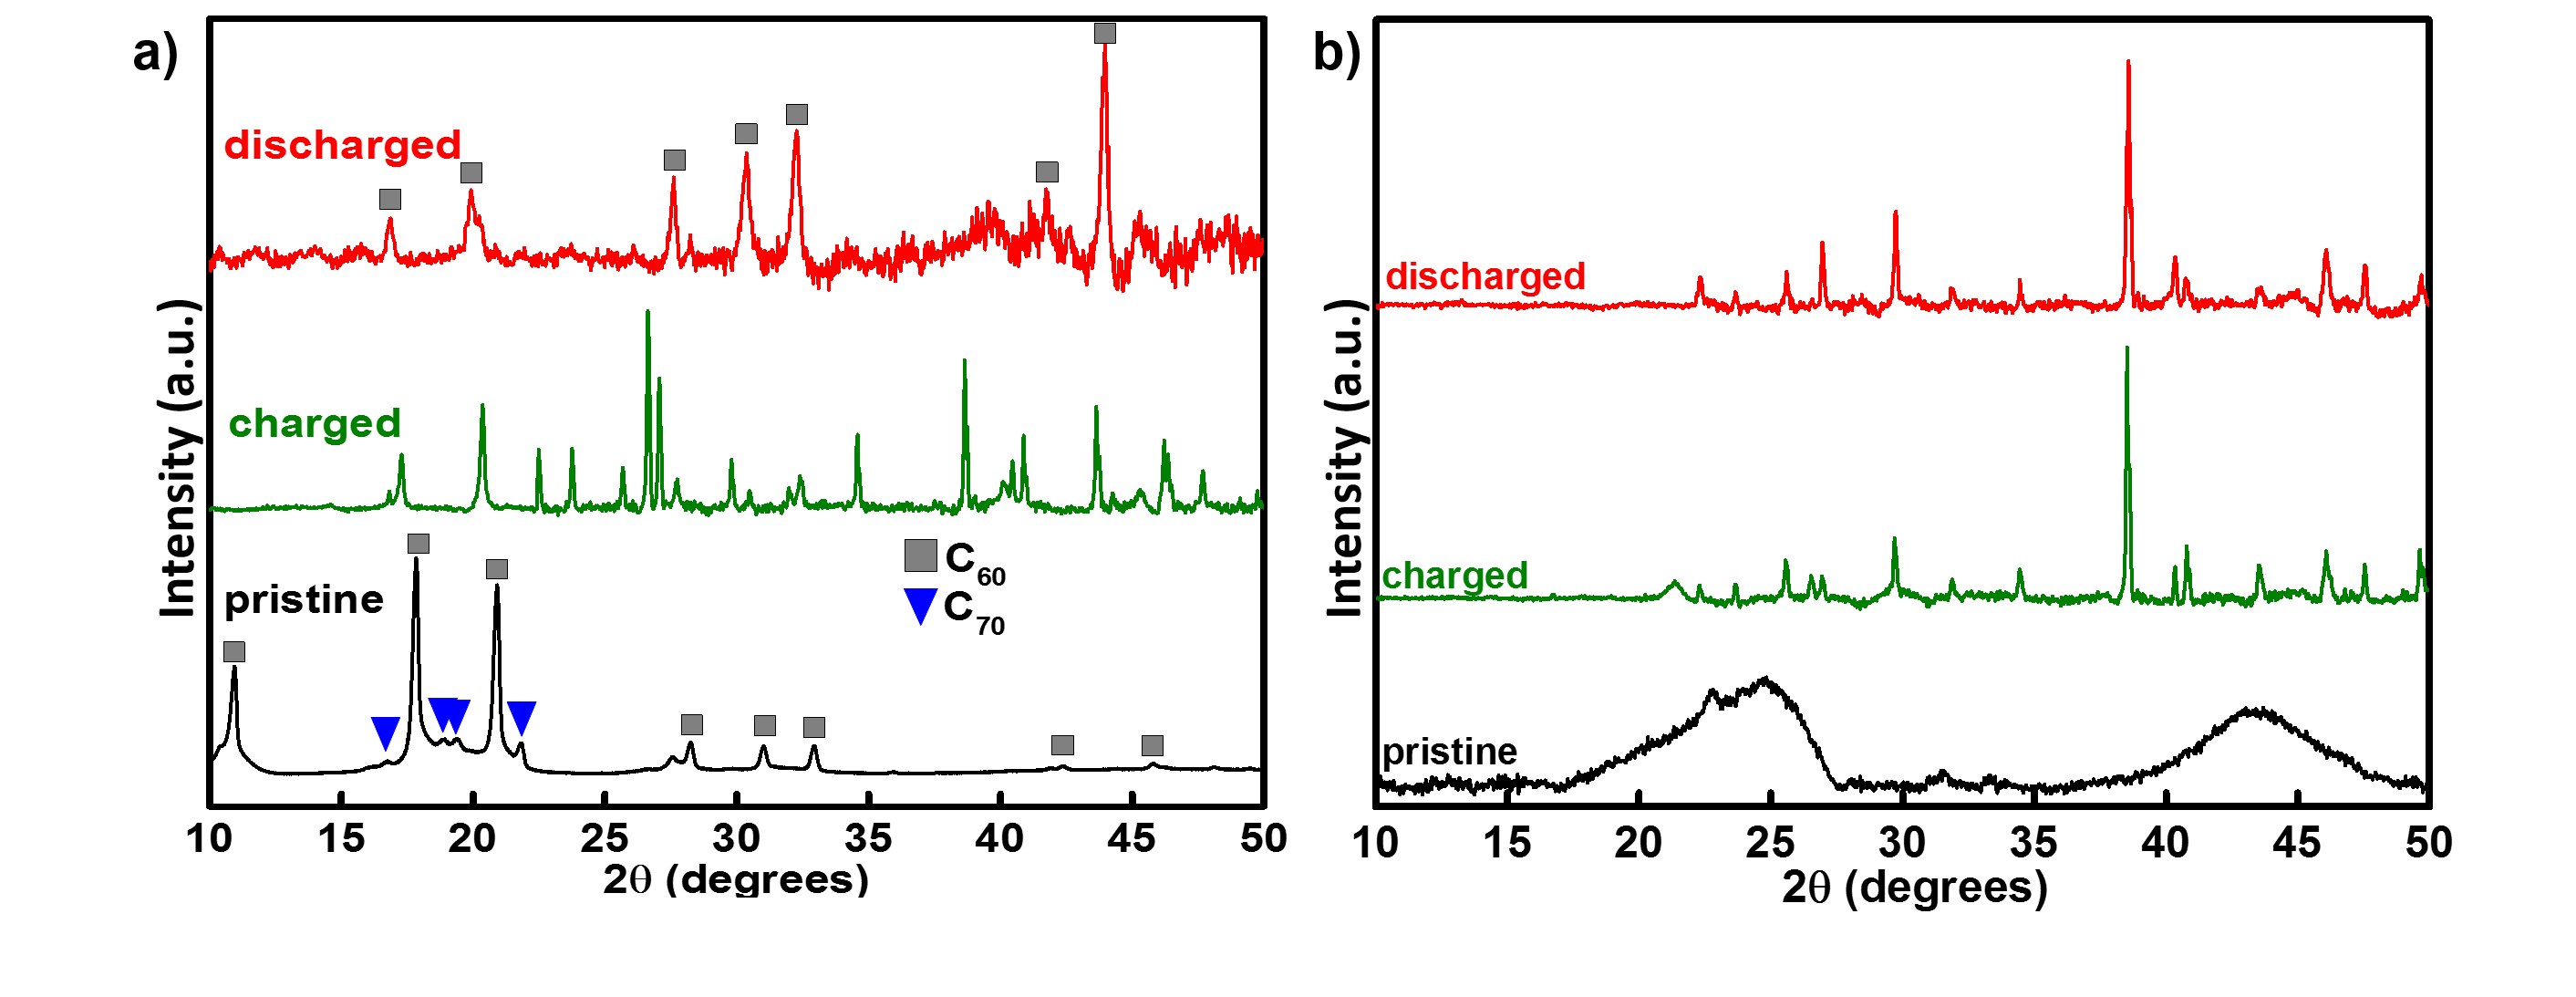
\includegraphics[width=\textwidth]{fig/XRD}
    \caption{X-ray diffraction (XRD) patterns of a) CFEx and b)human hair cathodes to study changes in their lattice after galvanostatic cycles in a two-electrode setup against \ce{Al$^{3+}$/Al} with characteristic peaks marked for \ce{C60} (in grey boxes) and \ce{C70} (in blue inverted triangles).}
  \label{fig:XRD}
\end{figure}

\begin{figure}%[tbh!]
  \centering
  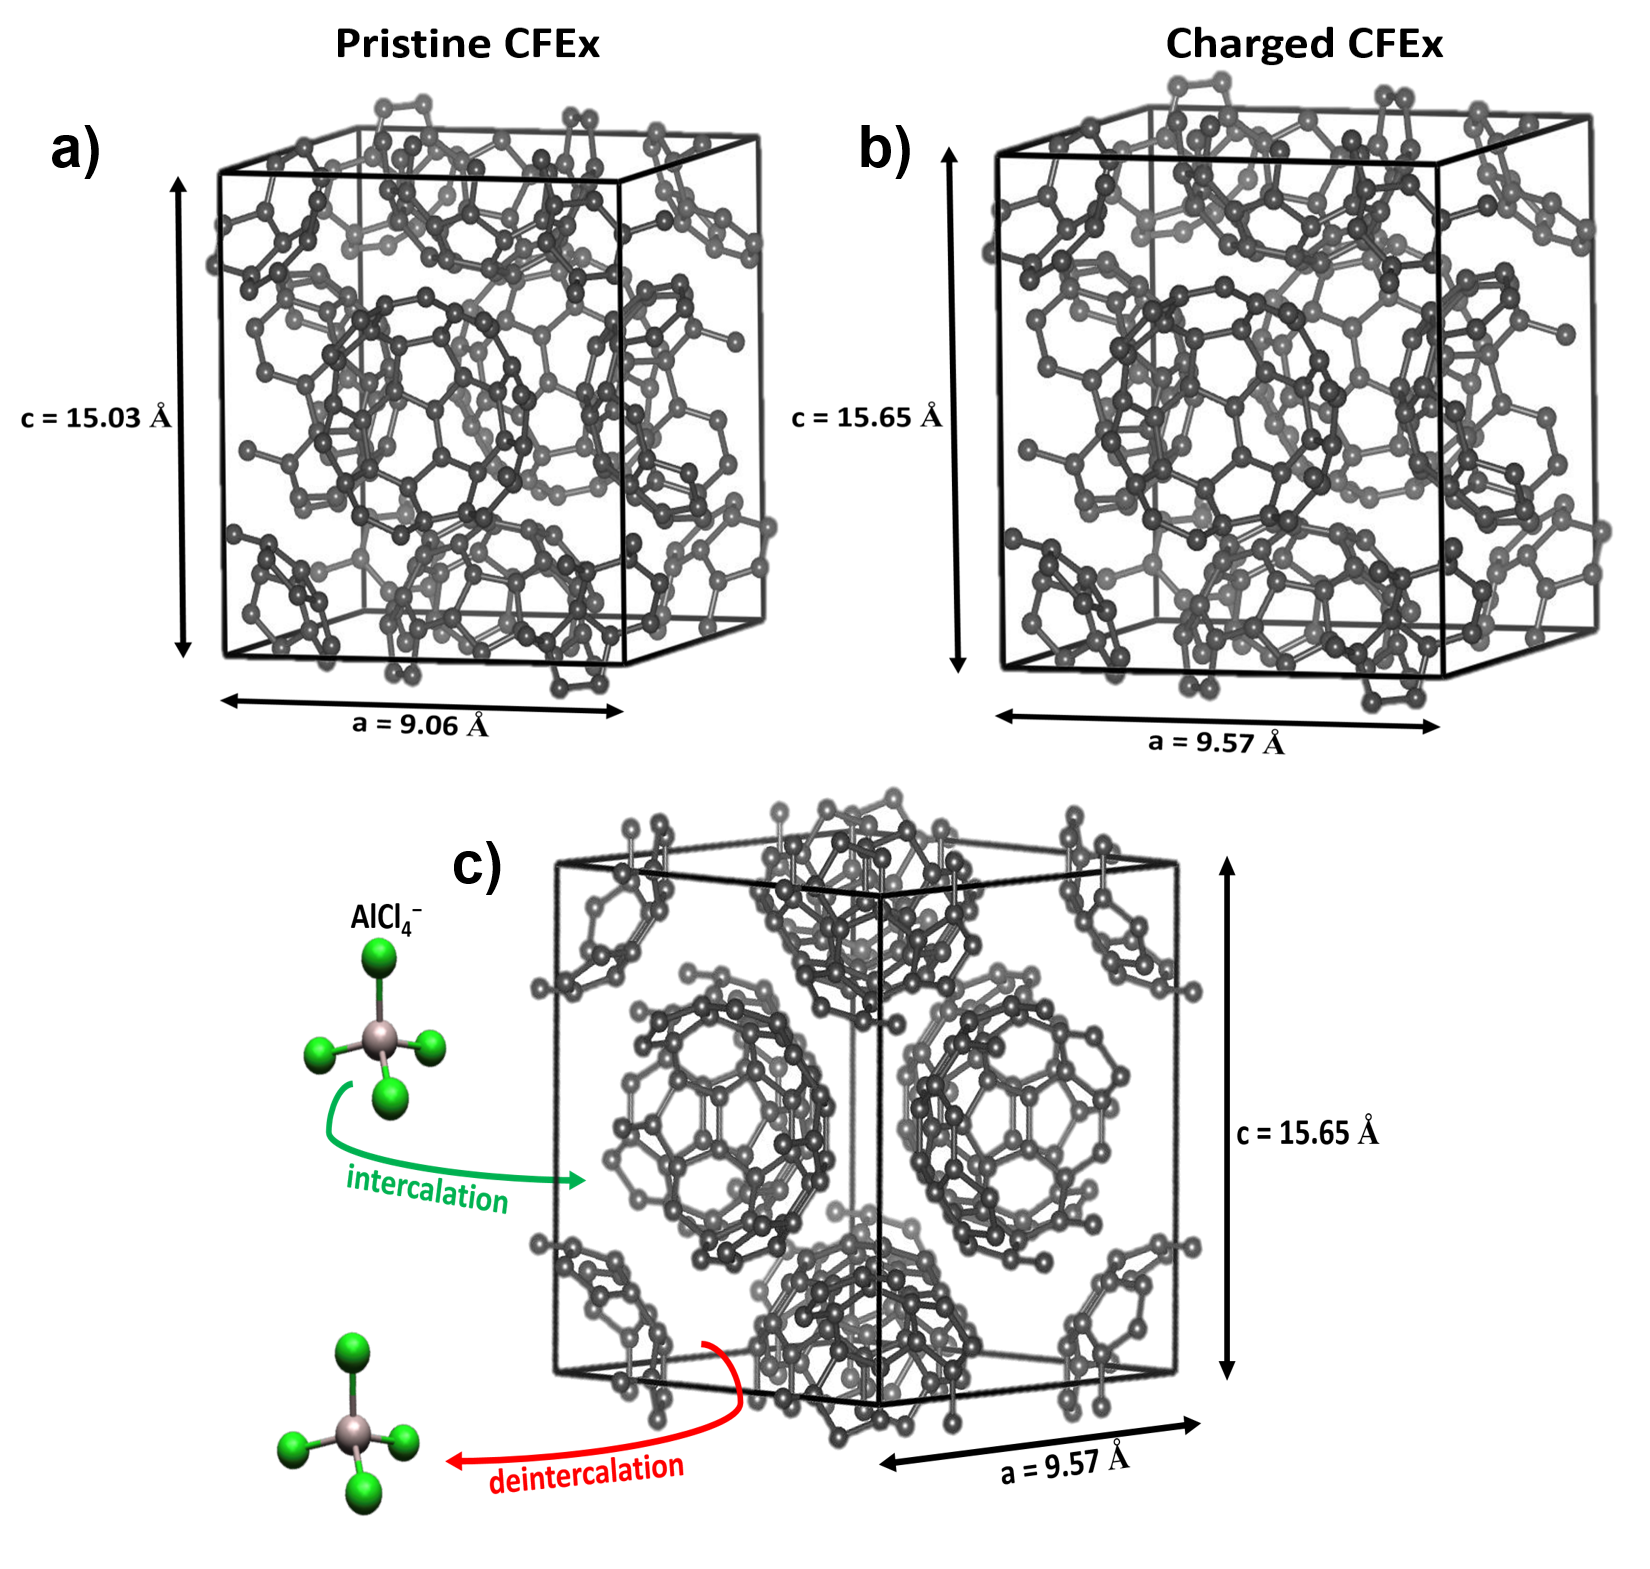
\includegraphics[width=\textwidth]{fig/cfexcrys}
    \caption{Changes in the lattice parameters of a \ce{C60} unit cell. a) Pristine \ce{C60}unit cell, b) charged \ce{C60}unit cell with increased parameters suggesting a uniform shift in the lattice after charge/discharge. c) Expected intercalation sites of \ce{AlCl4-} ions in the unit cell.}
  \label{fig:cfexcrys}
\end{figure}

XRD patterns of human hair cathodes were inconclusive (Figure \ref{fig:XRD}b)). The pristine cathode displayed broad peaks that confirmed a structure that was amorphous and highly porous. However, the material became more symmetrical and crystalline after cycling. Charged and discharged cathodes exhibited similar looking patterns implying no change in the newly formed crystal lattice during cycles. It has to be noted that the presence of crystallinity in an active material does not limit the surface-based charge storing capacity \cite{kim_synthesis_2006, jow_factors_2018}. Further analysis is required to investigate this unique behaviour and establish its mechanism.\\
To determine the different bonds and environments existing in all the carbon-based cathodes, XPS spectra of the carbon 1s orbital of all pristine cathodes is shown in Figure \ref{fig:XPSC}. Hair, hemp fibers and SPCB had similar looking peaks for the 1s orbital. All three cathodes displayed peaks for sp$^2$ C-C/ C-H, C-O/ C-OH, O-C=O/ C=O and C-F bonds. Since hair is mainly composed of a protein called keratin (Figure \ref{fig:keratin}), it can be deduced that multiple chemical environments of carbon, shown in Figure \ref{fig:XPSC}a), are derived from Keratin. Sulphide bonds are an essential part of this protein and a C-S binding energy was observed at 286.94 eV (blue peak).

\begin{figure}
  \centering
  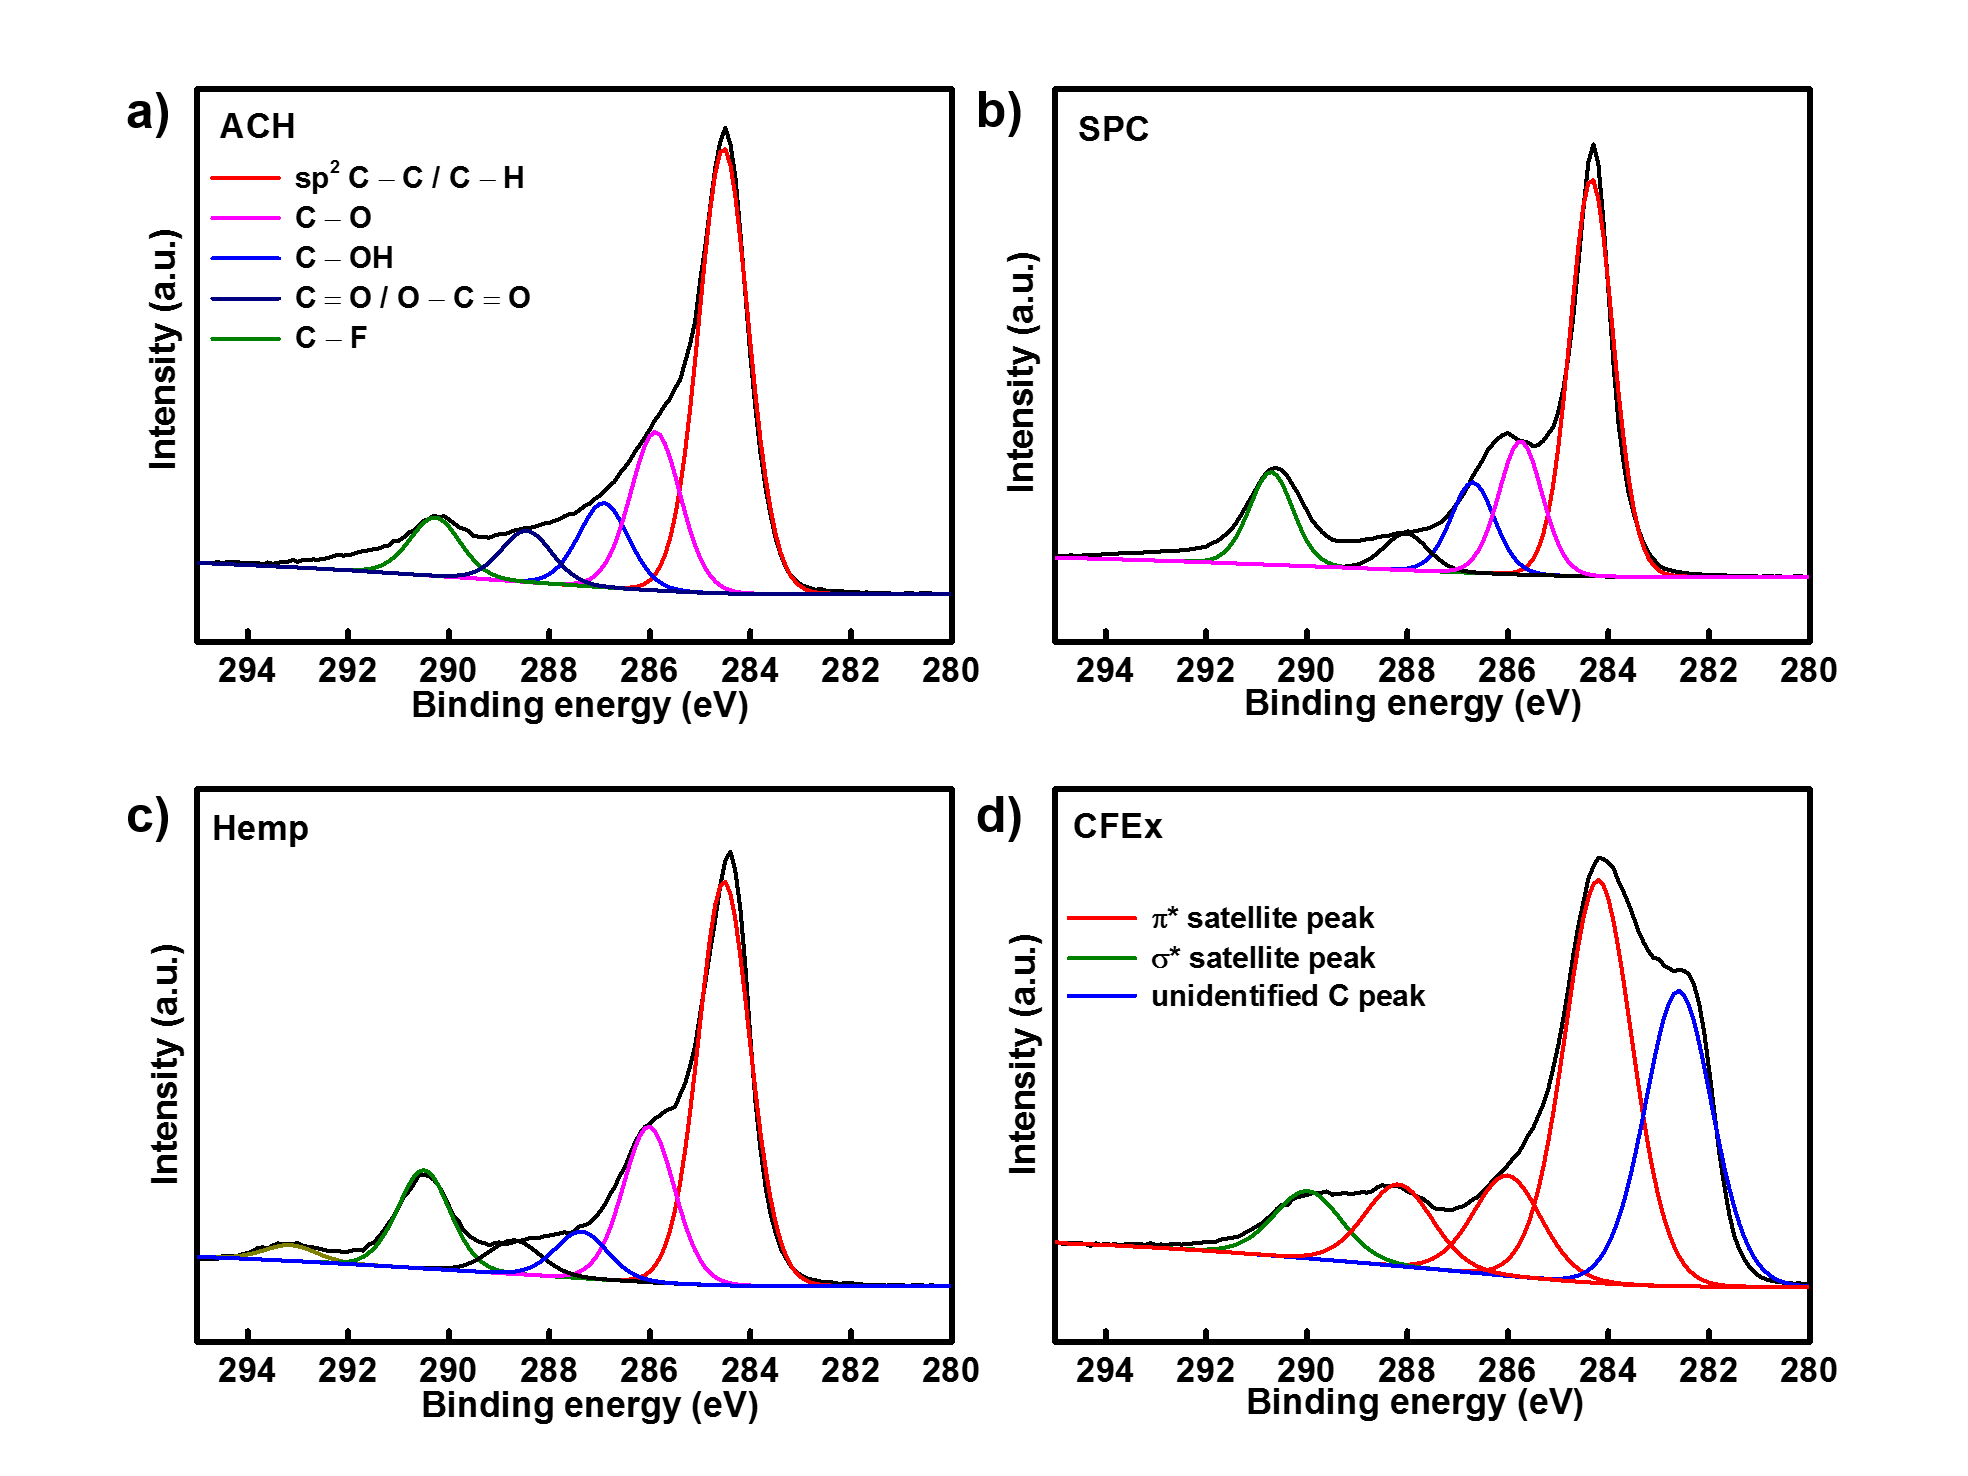
\includegraphics[width=\textwidth]{fig/XPSC}
    \caption{Carbon 1s XPS spectra of pristine a) hair, b) Super-P, c) hemp fibers and d) CFEx cathodes. While AC from human hair (ACH), hemp fibers and Super-P contain carbonyl functional groups, CFEx cathodes have symmetrical looking $\pi$* and $\sigma$* satellite peaks.}
  \label{fig:XPSC}
\end{figure}

\begin{table}
\caption{Carbon 1s peaks for various binding energies.} \label{table2}
\begin{tabular}{|cccccccc|}
\hline
Active & C-H/ & C-O/ & C=O/ & C-F & Pyrrolic N/ & aliphatic C-O & aromatic C=O\\
material & C-C & C-OH & O-C=O & & Pyridinic N & & \\
\hline
Human hair & 284.5 eV & 285.8 eV & 288.4 eV & 290.2 eV & 400.2 eV/ & 533.0 eV & 531.2 eV\\
& & & & & 398.3 eV & & \\
CFEx & 284.2 eV & 286.0 eV & 288.2 eV & 290.0 eV & 399.3 eV & 531.3 eV & 530.2 eV\\
Hemp fibers & 284.5 eV & 286.0 eV & 288.7 eV & 290.5 eV & 400.3 eV & 532.9 eV & 531.4 eV\\
SPCB & 284.3 eV & 286.7 eV & 288.0 eV & 290.7 eV & 400.2 eV & 532.8 eV & ---\\
\hline
\end{tabular}
\end{table}

Functional groups that contain oxygen, such as carbonyl and ester groups, improve the wettability of a material. This increases the availability of the active surface area as more electrolyte ions can interact with the material's surface \cite{younesi_analysis_2015}. SPCB is produced by partial oxidation of petrochemical precursors \cite{gnanamuthu_electrochemical_2011}. A perfect graphite surface containing only carbon atoms, without heteroatoms like oxygen and sulfur, would give a very well-ordered structure. The presence of impurities such as carbonyl groups creates defects resulting in a less graphitic and more amorphous structure \cite{hao_carbonaceous_2013} and peaks at 288.0 eV for -CO bonds in AC and SPCB cathodes confirming this observation. The presence of these defects was also observed in the form of D-bands in their Raman spectra (Figure \ref{fig:raman}). However, spectra for the C 1s orbital of CFEx were uniquely different due to the presence of several highly symmetrical peaks. The presence of $\pi$ electrons on its surface resulted in  multiple $\pi$ satellite peaks, which are typical in a \ce{C60} molecule \cite{skryleva_xps_2016}. These peaks appear in both high (in green) and low energy ranges (in red) \cite{erbahar_spectromicroscopy_2016, poirier_carbon_1993}. 

Figure \ref{fig:XPSON}a)-d) shows various binding energies for the oxygen 1s orbital. In addition to enhancing the wettability of a material \cite{li_effect_2011, oh_oxygen_2014}, oxygen-containing surface functional groups can provide pseudo-capacitance by reacting with electrolyte ions \cite{bleda-martinez_role_2005}. This might be another reason why aluminium-hair batteries performed better than the others. Due to its enhanced wettability, the active material was more exposed to the chloroaluminate ions. Figure \ref{fig:XPSoverall} displays the overall spectra of all tested cathodes. Table \ref{table1} summarises all the functional groups with their respective binding energies for all tested cathode materials in this project.

\begin{figure}
  \centering
  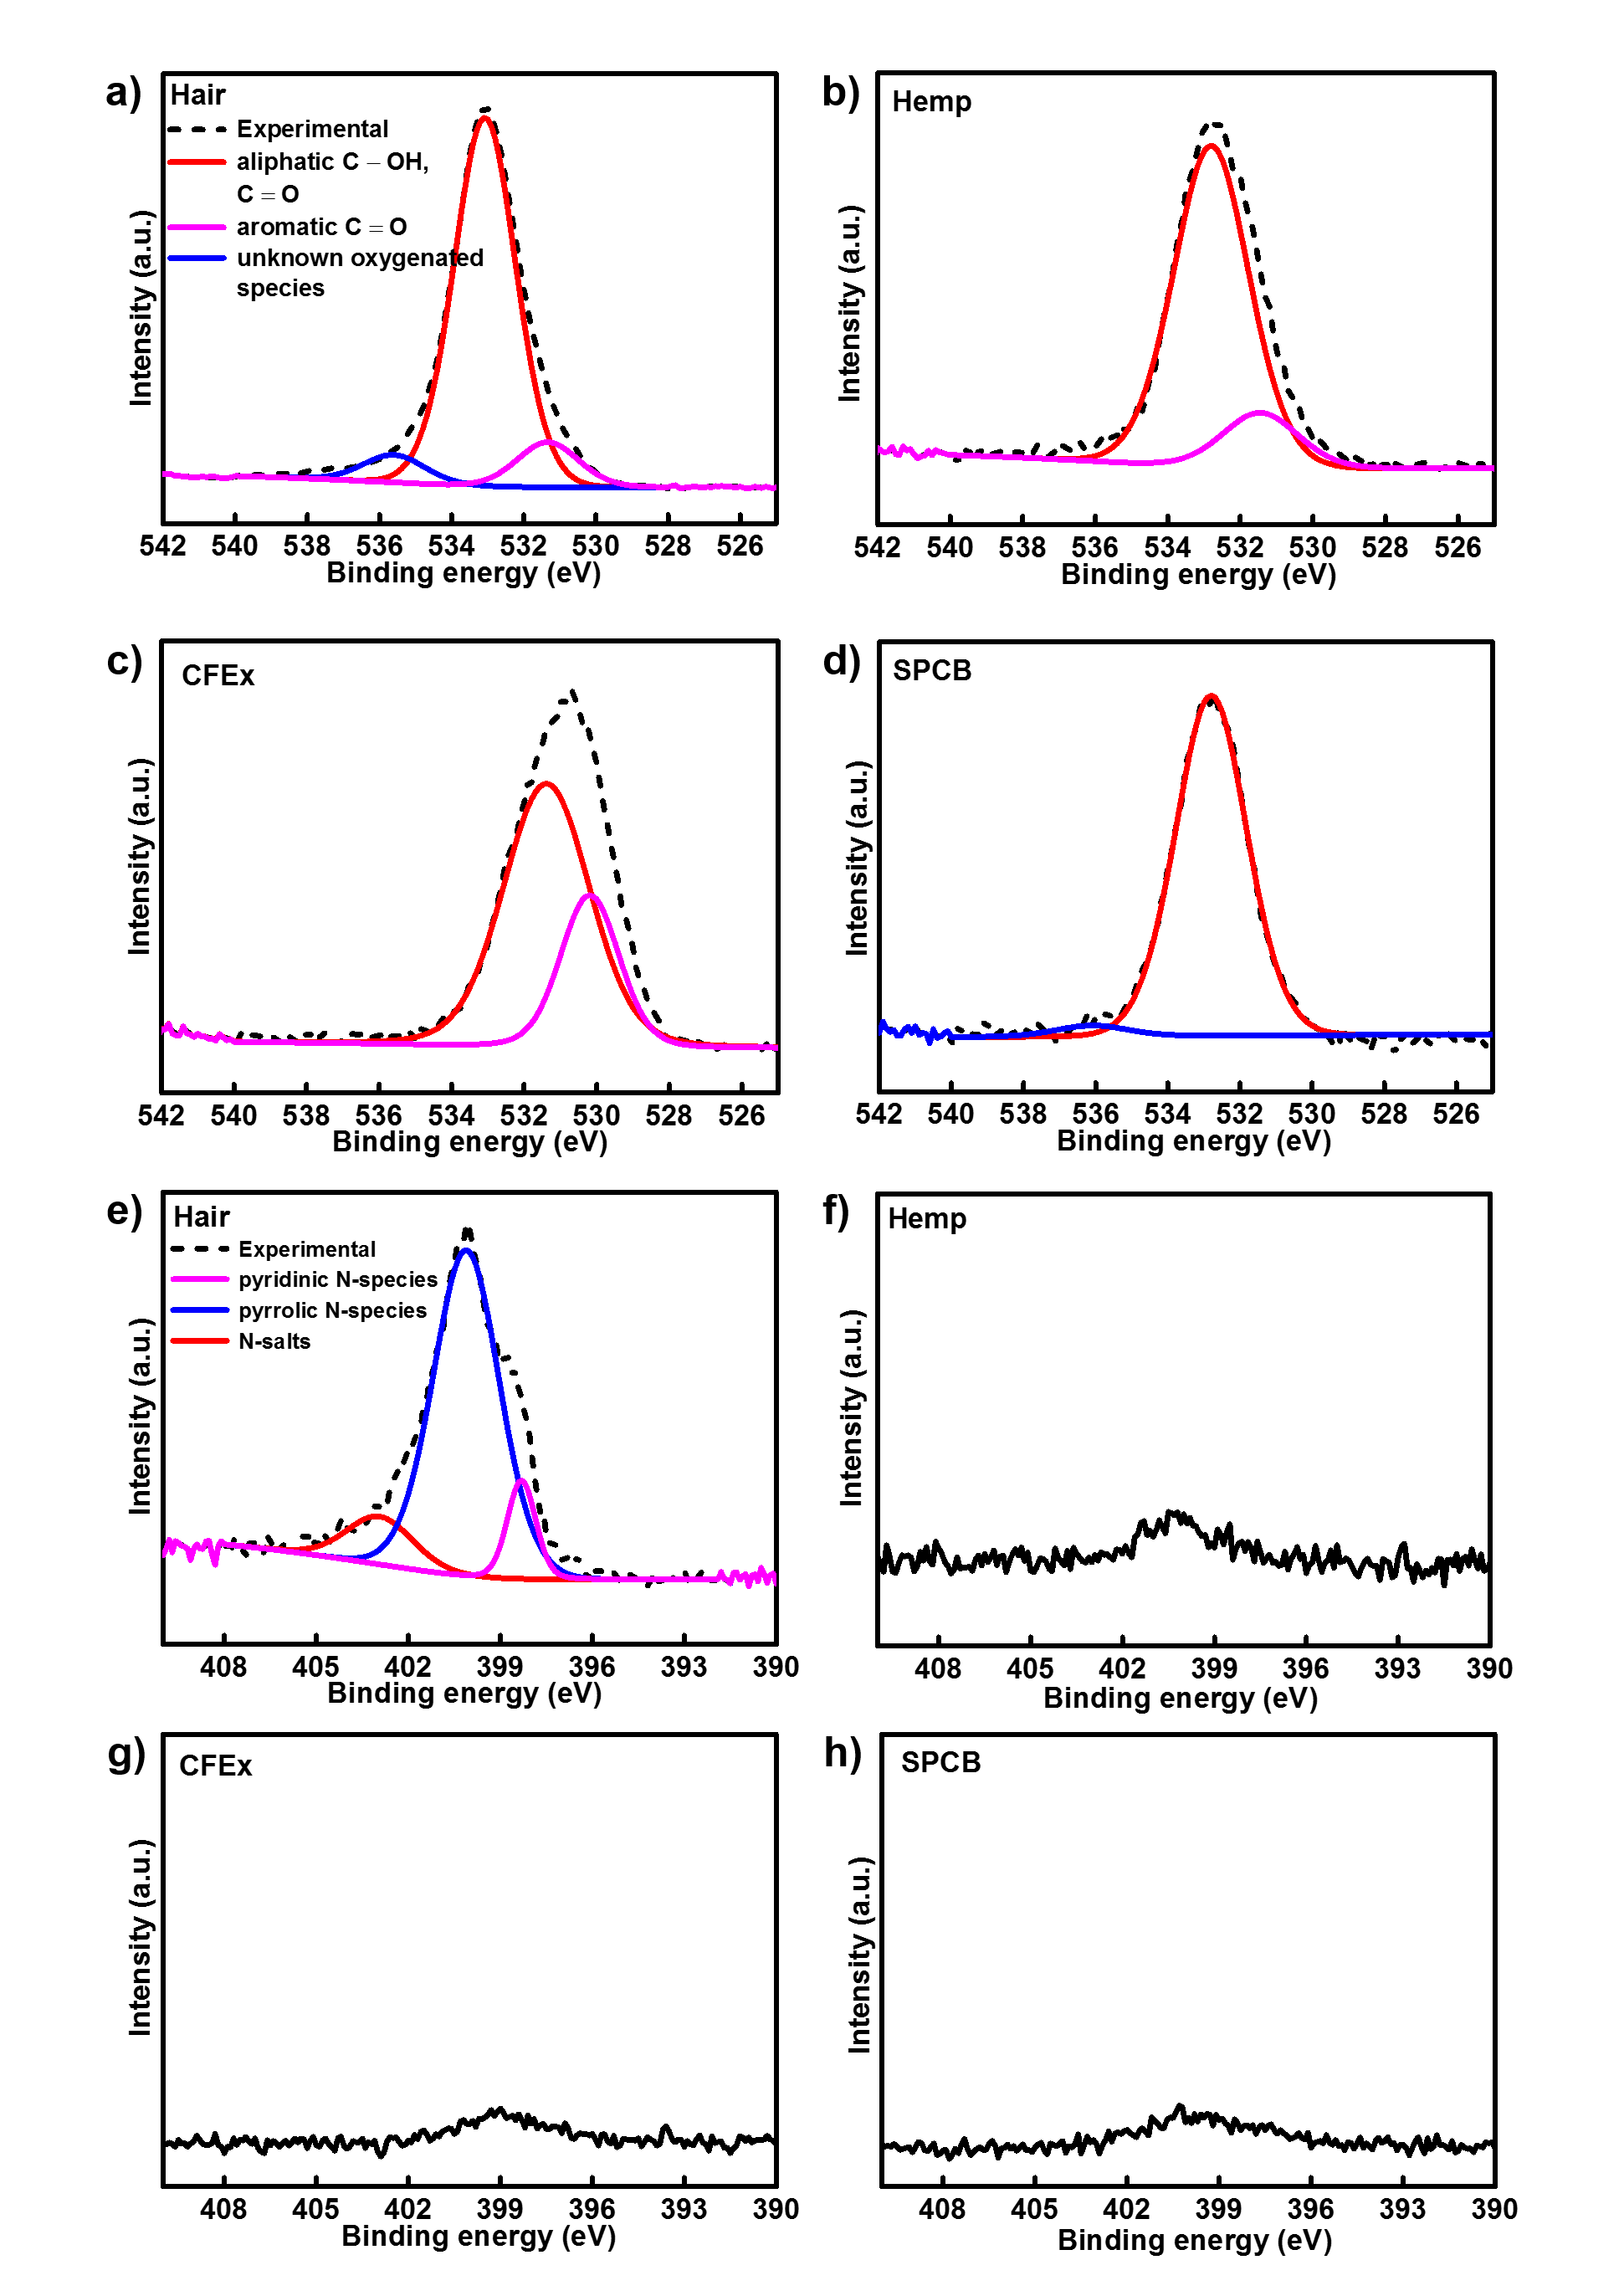
\includegraphics[width=0.8\textwidth]{fig/XPSON}
    \caption{XPS spectra of O 1s orbital for a) AC from human hair (ACH), b) hemp fibers c) CFEx and d) SPCB cathodes. Hair and hemp fibers contained significant amounts of aliphatic (red) and aromatic (pink) C=O groups  compared to CFEx and SPCB. Binding energies for N 1s orbital of e) hair, f) hemp fibers g) CFEx and h) SPCB cathodes. Human hair displayed distinct binding energies for pyridinic and pyrrolic N-species; hemp fibers, CFEx and SPCB had smaller amounts of surface proteins.}
  \label{fig:XPSON}
\end{figure}

\begin{figure}%[th!]
\centering
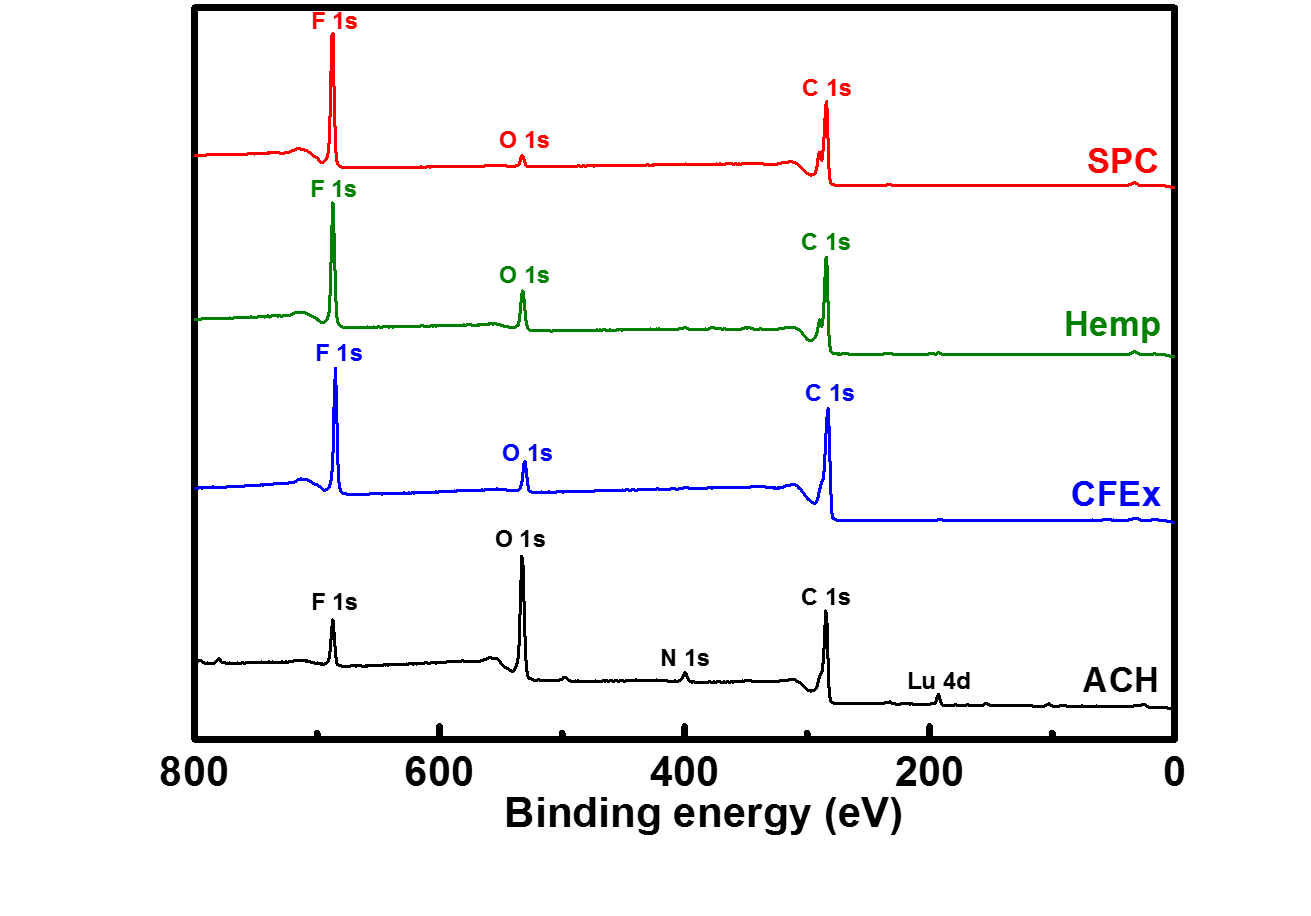
\includegraphics[width=\textwidth]{fig/XPSoverall}
\caption{Overall spectra of human hair (black), hemp fibers (blue), CFEx (green) and Super-P(red).}
\label{fig:XPSoverall}
\end{figure}

\begin{table}
\caption{Comparing battery metrics of all carbon-based cathodes tested in this work} \label{table1}
\begin{center}
\begin{tabular}{|lccc|}
\hline
Active material  & {\textbf{Specific capacity}} & {\textbf{Cell efficiency}} & {\textbf{Cell voltage}}\\
 & {\textbf{(mAh g$^{-1}$)}} & {\textbf{(\%)}} & {\textbf{(V)}}\\
\hline
Human hair &  102 & 97 & 1.9 \\
Fullerene mix &  78 & 85 & 1.7 \\
Hemp fibers & 49 & 75 & 1.8 \\
SPCB & 46 & 40 & 1.5 \\
\hline  
\end{tabular}
\end{center}
\end{table}

Lastly, to confirm whether AC derived from human hair is a psedocapacitive material, cyclic voltammograms of all cathodes at a scan rate of 10 mV s$^{-1}$ were compared. Figure \ref{fig:CV}a)-e) showed that human hair batteries resulted in a more rectangular, capacitor-like CV curve. However, redox processes were noticeable at a scan rate of 10 mV s$^{-1}$ and tiny redox peaks were visible in Figure \ref{fig:CV}b) at 1.8 and 2.1 V during charging and 1.1 and 1.9 V during discharge. At a higher scan rate (50 mV s$^{-1}$), the redox peaks disappeared and the material displayed an ideal capacitor-like CV curve, shown in Figure \ref{fig:hair50mVs} \cite{guan_capacitive_2016, dupont_separating_2015}. This happens because at a higher scan rate, the diffusion layer forms very close to the electrode and as a result of which higher current is recorded hiding the redox peaks. Although redox peaks were observed for CFEx (at 1.8 V during charging and 1.5 during discharging, which corresponds to the discharging plateau at $\sim$1.5 V) and others (Super-P: 1.8 V during charge and 1.9 and 0.9 V during discharge, hemp fibres: 1.1, 1.2 and 0.8 v during charge and 1.98 and 0.38 V during discharge), the measured current for the Super-P and hemp fibres was very low (negligible compared to human hair). At such low currents, it becomes impossible to draw conclusions about the reduction/oxidation reactions taking place and the stability of the species resulting from the electron transfer. 

 \begin{figure}
  \centering
  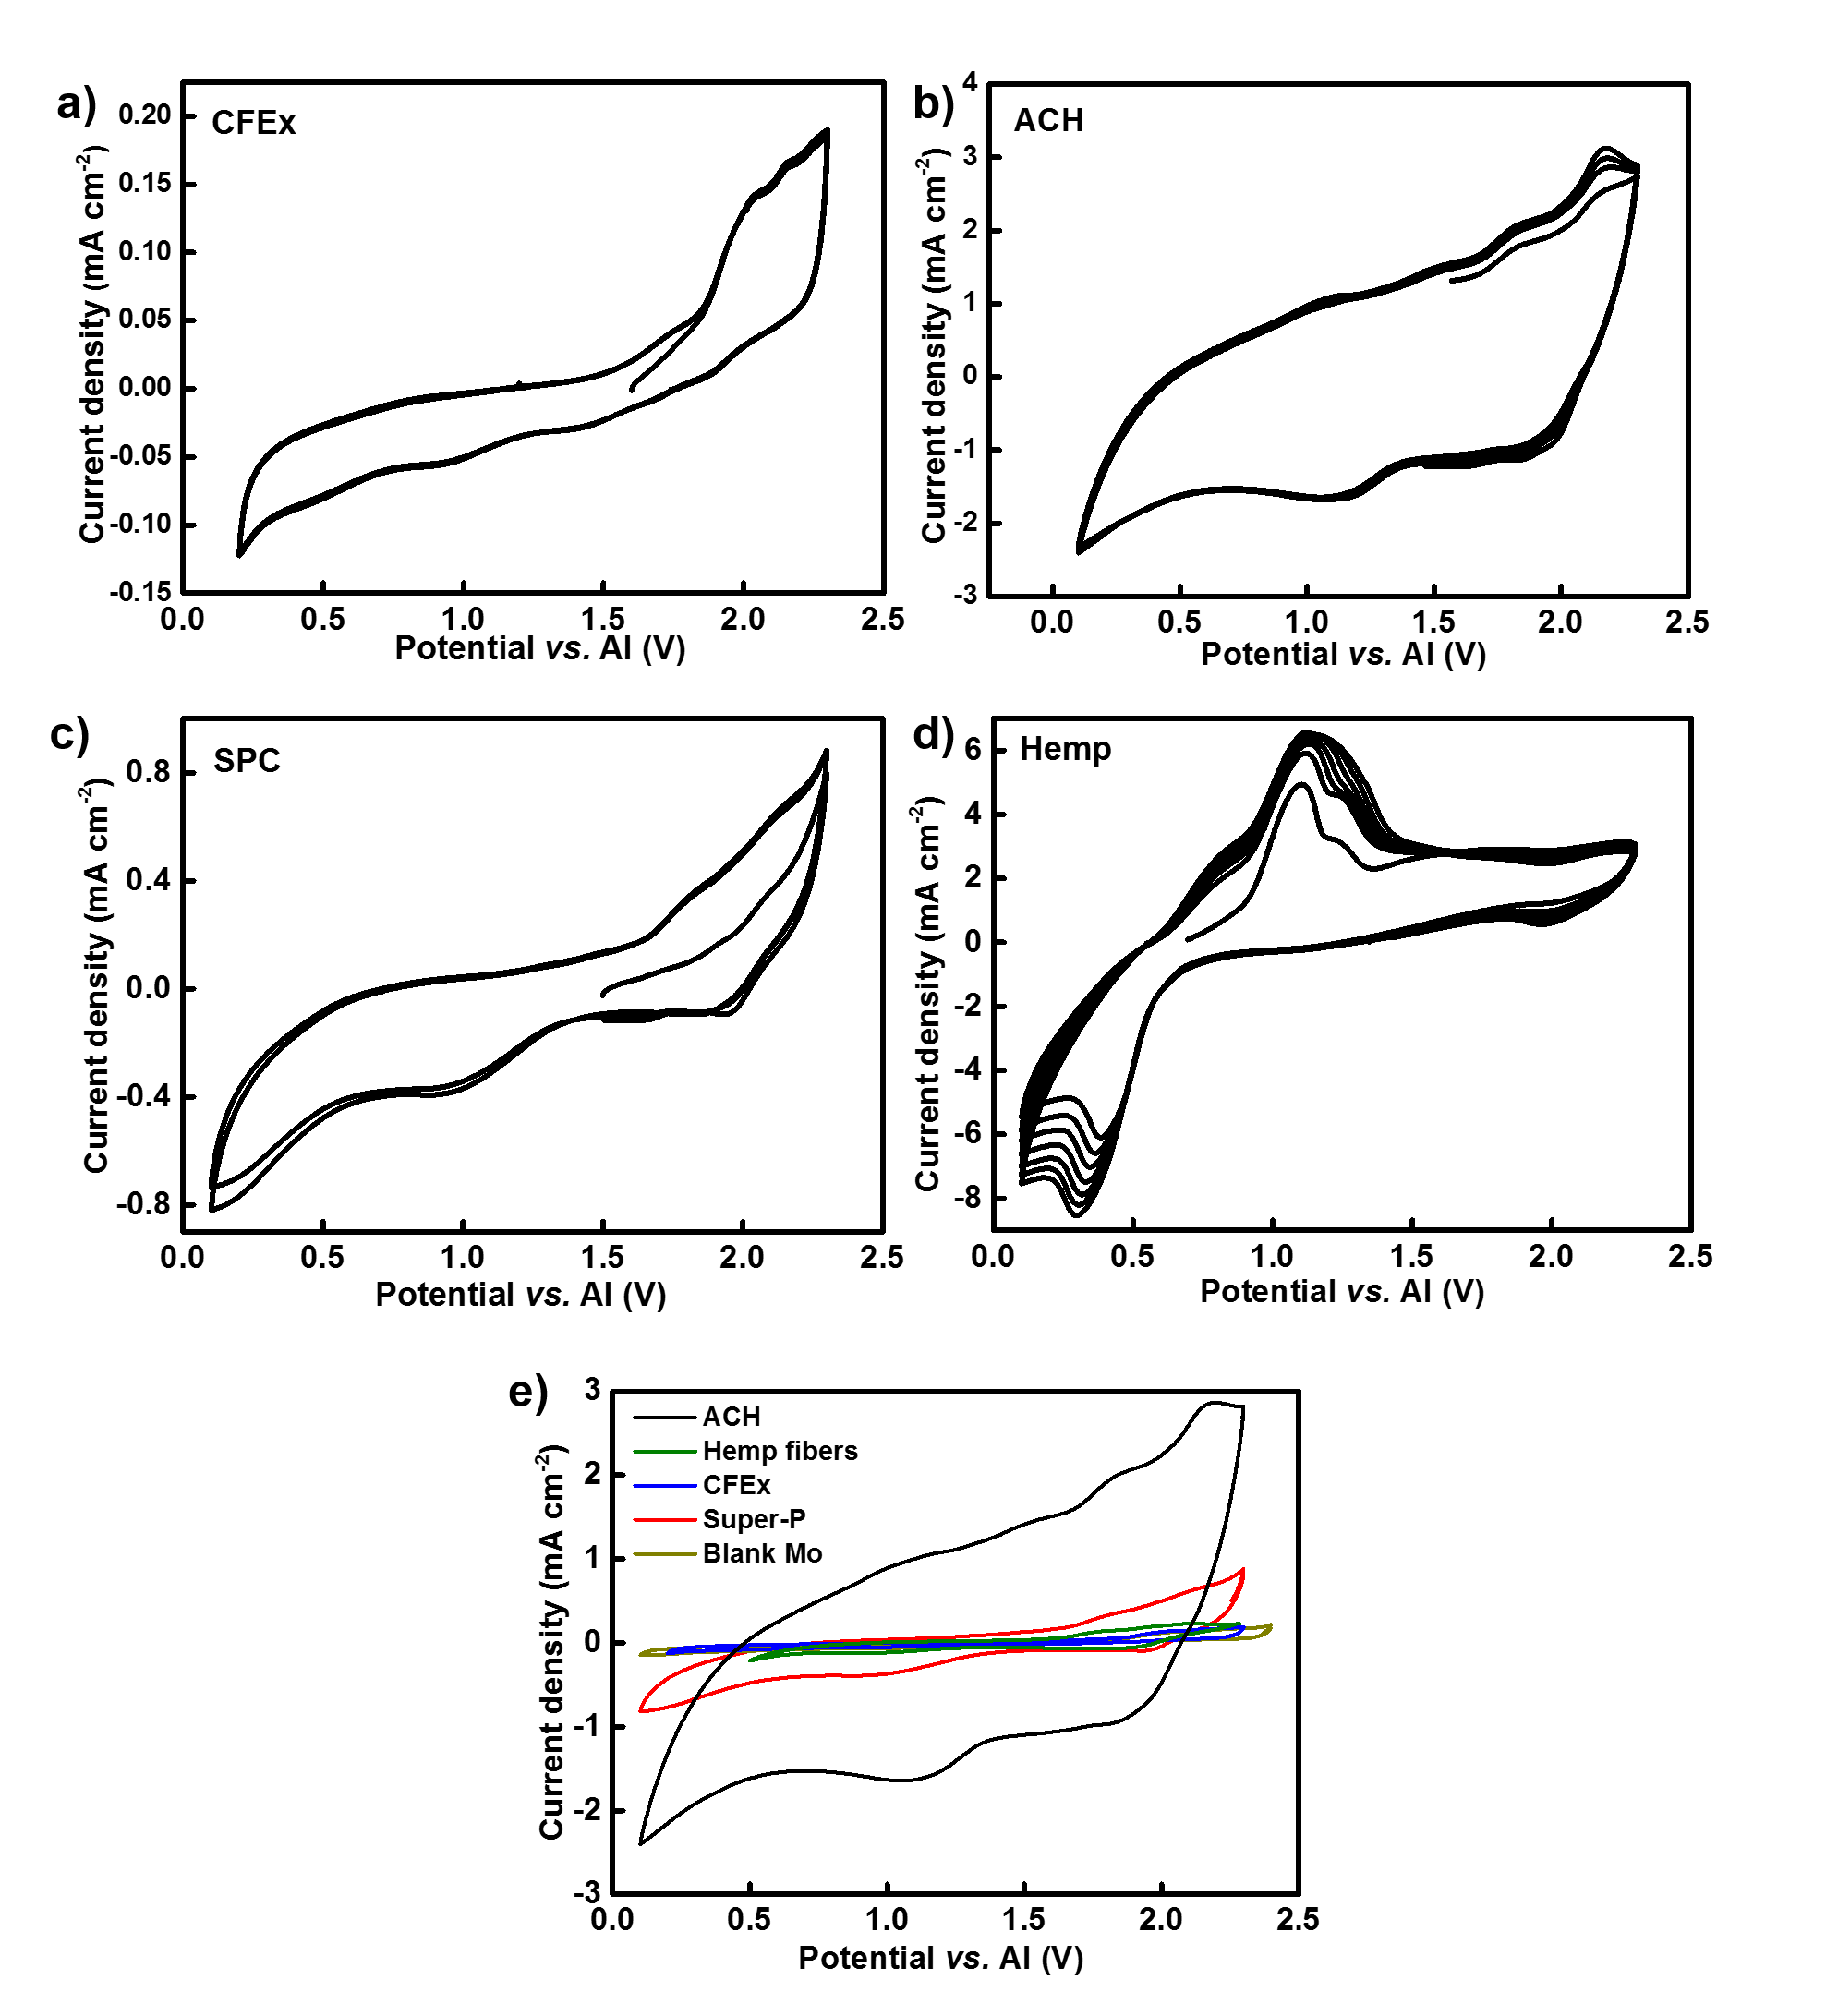
\includegraphics[width=\textwidth]{fig/CV}
    \caption{Cyclic voltammograms of a) CFEx, b) AC from hair, c) Super-P and d) hemp fibers cathodes at a scan rate of 10 mV s$^{-1}$ against \ce{Al3+}/Al as a counter/reference electrode in a two-electrode setup. ACH (activated carbon from hair) cathode observed a larger CV area than other cathodes, which comes from an additional pseudocapacitance, adding capacity to the system.}
  \label{fig:CV}
\end{figure}

\begin{figure}%[th!]
\centering

\includegraphics[width=\textwidth]{fig/hair50mVs}
\caption{Cyclic voltammogram of ACH at a scan rate of 50 mV/s in a two electrode setup against \ce{Al3+}/Al showing a capacitor-like behaviour with no visible oxidation-reduction peaks unlike Figure \ref{fig:CV}b, where redox peaks were observed.}
\label{fig:hair50mVs}
\end{figure}

\newpage
\section{Conclusion}
In summary, AC derived from human hair proved to be the best carbon-based cathode among all the tested materials in this work, with a specific capacity of 100 mAh g$^{-1}$ at a potential of 1.9 V with a CE of $\sim$90$\%$. Intercalation and deintercalation of \ce{AlCl4-} takes place in the very few graphitic layers. It was found that in CFEx \ce{AlCl4-} anions migrate in and out of the gaps in between the fullerenes changing its structure and slightly expanding the crystal lattice during charging (Figure \ref{fig:cfexcrys}). Moreover, fullerenes maintain their structural integrity and CE throughout the cycles. Hemp fibers and Super-P on the other hand, have a highly amorphous structure, which degraded after every cycle, resulting in a low capacity value. Figure \ref{fig:CFExACHlong} shows the 50th cycle measurement for Al/hair and Al/natural graphite cell. It not only displays a higher specific capacity than conventional graphite, but also a high battery voltage of 1.92 V with an energy density of 202 Wh kg$^{-1}$. The high battery performance can be attributed to the porosity of the material combined with its high surface area and the presence of hetero-atoms. The cumulative effect of the surface-based non-Faradaic and redox Faradaic contributions lead to the material achieving higher capacities than the other materials.

\begin{figure}%[h!]
  \centering
  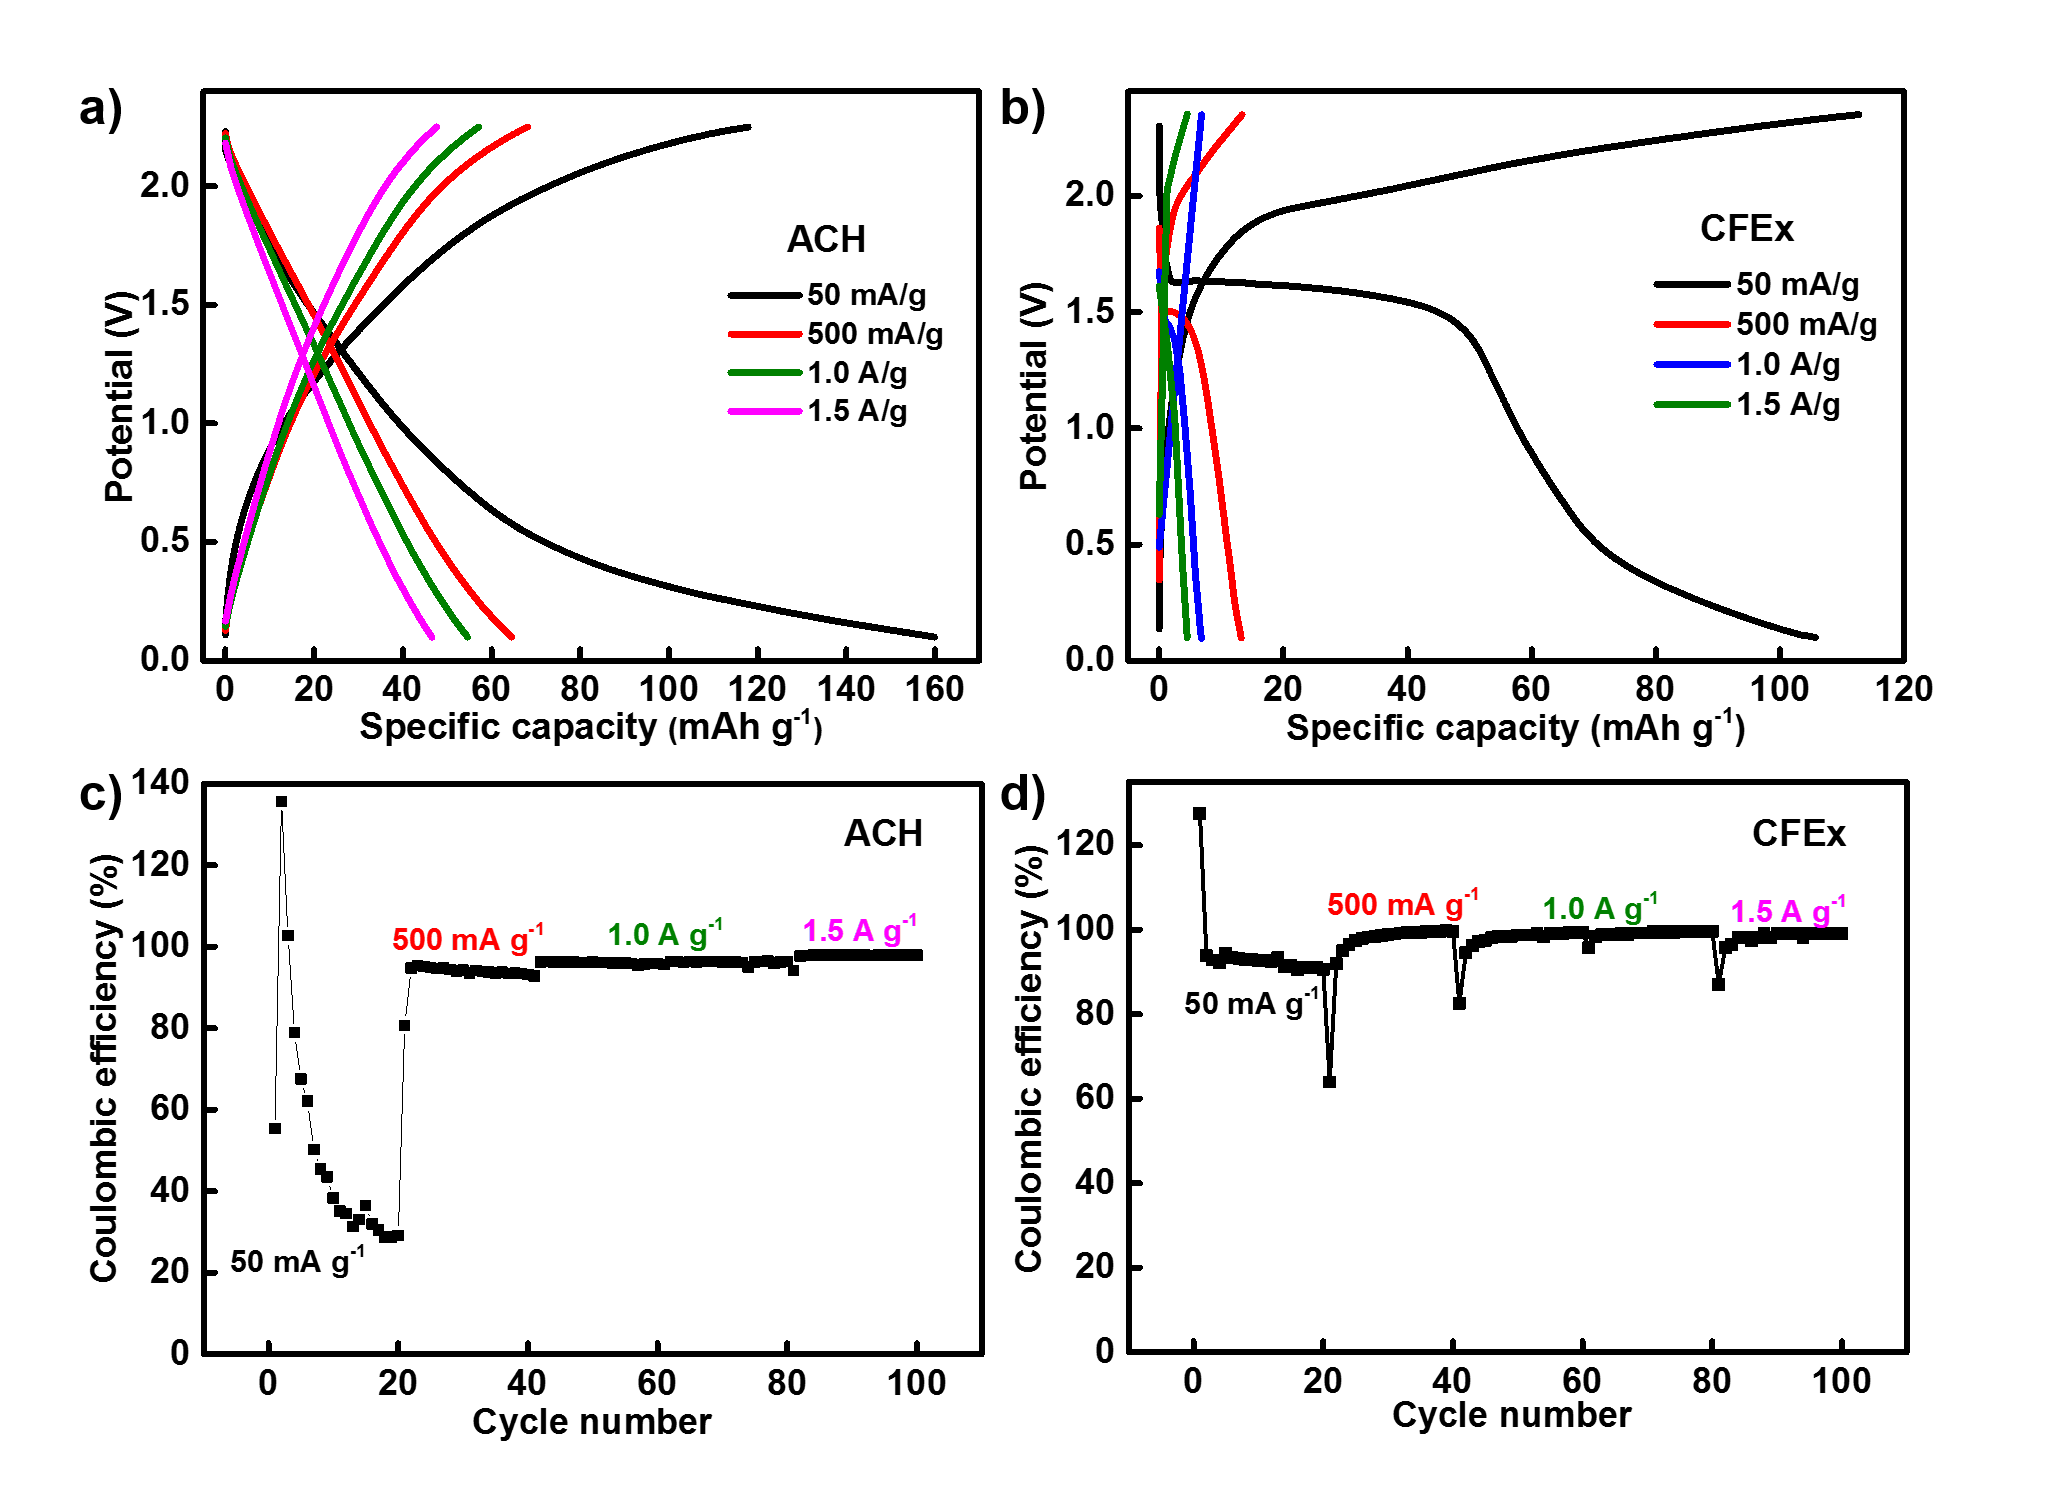
\includegraphics[width=\textwidth]{fig/CFExACHlong}
    \caption{Discharge capacities of a) ACH and b) CFEx cathodes at current rates of 50 mAg$^{-1}$, 500 mAg$^{-1}$, 1.0 Ag$^{-1}$ and 1.5 Ag$^{-1}$ along with their CEs. }
  \label{fig:CFExACHlong}
\end{figure}

\newpage

\section{Experimental Section}
\subsection{Chemicals}
\subsubsection*{AC from human hair}
AC derived from human hair was prepared by obtaining hair from the barber shops located in Wellington. The hair was initially cut into small pieces and washed thoroughly using isopropanol (IPA) to get rid of any chemicals from shampoo and conditioners. The samples were then dried at 100 $^{\circ}$C for 12 hours. The dried hair was then burnt in Ar atmosphere at 300 $^{\circ}$C for 90 minutes. The pre–carbonized sample was then mixed with NaOH (Sigma-Aldrich) in a mass ratio of 1:2. The sample was later carbonized at 750 $^{\circ}$C for 3 hours in presence of Ar. The product obtained was repeatedly washed with hot milli-q water to remove any traces of sodium from the sample, which was then dried at 80 $^{\circ}$C for 6 hours to obtain the final product.

\subsubsection*{AC from hemp fibers}
The material was provided by Carbon Valley and used as received.
\subsubsection*{Fullerene extract}
\ce{C60}/\ce{C70}, approx. 85\% \ce{C60}, 14\% \ce{C70}, and 1\% higher fullerenes, was purchased from SES research and used as received.
\subsubsection*{Super-P carbon black}
Super-P conductive carbon, 99+\% metals basis was purchased from Alfa Aesar and used as received

\subsection{Cathode preparation}
A slurry was prepared by mixing the active material (85$\%$ by wt.), 9$\%$ binder (PVDF, MTI Corp.) and 6$\%$ Super-P conductive carbon (99+$\%$ metals basis, Alfa Aesar) in N-methyl pyrrolidone NMP (anhydrous, 99.5$\%$, Sigma-Aldrich). To form the Super-P slurry, 94$\%$ (by weight) of Super-P (active material) and 6$\%$ (by weight) of the binder were mixed together in the solvent. The slurries was then doctor-bladed onto molybdenum foil, which was used as the current collector (thickness 0.1 mm, MTI Corp.). The coated sheets were dried in a vacuum oven at 120$^{\circ}$C for 12 hours to adhere the slurry on the substrate and fully evaporate the solvent. The specific loading of the slurry material ranged from 11-12 mg cm$^{-2}$ on each cathode. 

\subsection{Electrolyte preparation}
Anhydrous \ce{AlCl3} (Sigma-Aldrich) and EMImCl (97$\%$, Sigma-Aldrich) were mixed in a molar ratio of 1.3:1, at room temperature. EMImCl was baked in vacuum for 24 hours at 100$^{\circ}$C to remove residual moisture. Small aliquots of AlCl$_3$ was added to EMImCl after every few minutes. The ionic liquid was stirred for 2-3 hours until a clear brown liquid was obtained. Since the electrolyte is hygroscopic in nature, it was prepared in a N$_2$-filled glove box with <0.1 ppm H$_2$O/O$_2$. 

\subsection{Cell assembly}
PEEK (polyether ether ketone) cells were used for electrochemical measurements (Figure \ref{fig:PEEK}). Molybdenum rods were used as current collectors. It was seen previously that steel rods reacted with the electrolyte forming a green-colored substance on the cathode. The slurry coated on molybdenum foil was used as the cathode and placed at bottom of the cell. Two glass microfibers (Grade GF/F, Whatman) were used as separators. 80$\mu$l of the electrolyte was used to wet the separator. Al foil (thickness 0.1 mm, 99$\%$, GoodFellow) used as an anode and placed on top of the separator. It was assembled in a N$_2$-filled glove box. The cell was then sealed and wrapped with a paraffin film to avoid any air or moisture contact. Since this was a two-electrode setup, Al foil was used as both counter and reference electrode. The cell was taken out of the glove box and electrochemical measurements were performed. 

\subsection{Activation of carbon (hair)}
In this reaction, NaOH was reduced to free metal, Na. These atoms in turn expanded the carbon matrix after intercalating into the carbon structure. Increased temperature (750$^{\circ}$ C) forced the  atoms out of the carbon matrix, thus creating micropores. Oxidation of carbon from oxygen atoms of the hydroxide group formed carbon dioxide (\ce{CO2}), providing routes for channeling the sodium atoms into the internal structure, resulting in a well-connected porous structure \cite{satish_macroporous_2015}. The calcinating temperature used here was 750$^{\circ}$ C. Figure \ref{fig:ACHsyn} displays a flowchart describing an AC synthesis. 

\section{Acknowledgement}
We thank Panya Thanwisai and Dr. Nonglak Meethong from Khong Kaen University, Thailand for their help with the synthesis of AC from human hair. 

% What is this figure doing here in the wild?
%\begin{figure}[tbh!]
 % \centering
  %
\includegraphics[width=\textwidth]{figures/GCDCall}
   % \caption{Chronopotentiographs (Voltage vs. Time) curves of all tested cathodes.}
  %\label{figures:GCDCall}
%\end{figure}

\bibliographystyle{unsrt}  % Something must be wrong here....
\bibliography{thesisref2} 

\end{document}
